%!TEX root = ./main.tex

%%**************************************************************
%%
%% DHBW Heidenheim - Template for Bachelor Thesis
%%
%% Bevor usisng this template please have a look at the REAMDME.md file
%%
%%**************************************************************

\input{ads/header}

\input{content/glossary}

\begin{document}

	% Cover
	\begin{spacing}{1}
		\input{ads/cover}
	\end{spacing}
	\newpage

	\pagenumbering{Roman}

	% Restriction notices
	\ifDocType{T2\_3100}{%
		% no restricition notices for semester paper
	}{%
		\input{ads/restrictionNotices}
		\newpage
	}%

	% Declaration
	\input{ads/declaration}
	\newpage

	% Abstract
	%!TEX root = ../main.tex

\pagestyle{empty}

% override abstract headline
\renewcommand{\abstractname}{Abstract}

\begin{abstract}

    Eine Progressive Web App (PWA) ist eine Website, welche eine Vielzahl an Charakteristika nativer Apps aufweist. Wie jede andere Website auch können PWAs mit JavaScript, HTML und CSS erstellt werden. Was sie in ihrer Nutzung jedoch von herkömmlichen responsiven Webseiten unterscheidet, sind app-spezifische Merkmale wie die Installierbarkeit, der Zugriff auf Geräteschnittstellen, die Verfügbarkeit im Offline-Modus sowie die Möglichkeit der Aktivierung von Push-Nachrichten.

    Dennoch können PWAs auch gegenüber nativen Apps einen entscheidenden Vorteil liefern. PWAs sind unabhängig von Plattformen. App-Entwickler stehen oft vor der Herausforderung, eine App in mehreren Programmiersprachen zu entwickeln, um sie für verschiedene Betriebssysteme und Geräte zur Verfügung stellen zu können. 
    
    Der daraus entstehende Aufwand soll mithilfe von PWAs minimiert werden. Eine Entwicklung in verschiedenen Programmiersprachen ist hierbei nicht nötig; die Verwendung von Website-Entwicklungs-Tools und -Bibliotheken ist ausreichend. Die Aufwandsminimierung soll dennoch nicht mit einer Einschränkung der vollumfänglichen Einsetzbarkeit auf allen Plattformen einhergehen. 
    
    Ob PWAs plattformübergreifend alle Ansprüche erfüllen können und reif genug sind, eine relevante Alternative zu nativen Apps darzustellen, soll in der Arbeit ermittelt werden.  

\end{abstract}
	\newpage

        % only page number in footer
	\pagestyle{plain}
	
	% space bevore chapter headline
	\RedeclareSectionCommand[beforeskip=\chapterMargin]{chapter}

	% Contents
	\begin{spacing}{1.1}
		\begingroup
		
		    % set subchapter depth
			\setcounter{tocdepth}{2}
			
			\tableofcontents
			\clearpage
		\endgroup
	\end{spacing}
	\newpage

	% Acronyms
	\cleardoublepage
    %!TEX root = ../main.tex

\addchap{\acronymsPhrase}

\begin{acronym}[YTMMM]
\setlength{\itemsep}{\parsep}

\acro{PWAs}{Progressive Web Apps}
\acro{PWA}{Progressive Web App}
\acro{JSON}{JavaScript Object Notation}
\acro{URL}{Uniform Resource Locator}
\acro{API}{Application Programming Interface}
\acro{DOM}{Document Object Model}
\acro{SPA}{Single Page Application}
\acro{SQL}{Structured Query Language}
\acro{CRUD}{create, read, update and delete}
\acro{HTTP}{Hypertext Transfer Protocol}
\acro{HTML}{Hyper Text Markup Language}
\acro{CSS}{Cascading Style Sheets}
\acro{REST}{Representational State Transfer}
\acro{RDBMS}{Relational Database Management System}
\acro{NoSQL}{Not only SQL}
\acro{BSON}{Binary JSON}
\acro{CLI}{Command Line Interface}
\acro{AVD Managers}{Android Virtual Device Manager}
\acro{IETF}{Internet Engineering Task Force}
\acro{VAPID}{Voluntary Application Server Identification}
\acro{APNs}{Apple Push Notification service}
\acro{TLS}{Transport Layer Security}
\end{acronym}


	% List of Figures
	\cleardoublepage
	\listoffigures

	%List of Tables
	\cleardoublepage
	\listoftables

	% List of Listings
	\cleardoublepage
	\lstlistoflistings
	\cleardoublepage

	\pagenumbering{arabic}
	
	\pagestyle{headings}

	%Content

%	\foreach \i in {01,02,03,04,05,06,07,08,09,...,99} {%
%		\edef\FileName{content/chapter/\i .tex}%
%			\IfFileExists{\FileName}{%
%				\input{\FileName}
%			}
%			{%
%				No chapter available
%			}
%	}
	%%%%%%%%%%%%%%%%%%%%% Einleitung %%%%%%%%%%%%%%%%%%%%%%%%%%%%%%
	%!TEX root = ../../main.tex

\chapter{Einleitung} \label{ch:Einleitung}
	%!TEX root = ../../main.tex

\section{Motivation} \label{se:Motivation}

Folgendes Szenario soll einen Einblick in die Vorteile von \ac{PWAs} geben. 

Ein junges Startup aus IT-Studenten hat eine Idee für eine Applikation und möchte diese umsetzen. Ihr Ziel ist es, diese Applikation an so viele Nutzer wie möglich zu verbreiten. Die Applikation soll demnach für folgende Plattformen verfügbar sein - siehe Tabelle \ref{plattformen}.

\begin{table}[!htb]
\begin{tabularx}{\textwidth}{|X|X|}
    \hline
    \textbf{Plattform} & \textbf{Programmiersprache} \\
    \hline
    \hline
    IOS & Swift \\
    \hline
    Android & Java oder Kotlin\\
    \hline
    MacOS & Swift \\
    \hline 
    native Windows & C++ oder C\# \\
    \hline
    Webbrowser & JavaScript, HTML und CSS \\
    \hline
\end{tabularx}
\caption{Plattformen und die dazu benötigten Programmiersprachen}
\label{plattformen}
\end{table}

Wie man anhand der Tabelle sehen kann, kommt eine Vielzahl an unterschiedlichen Programmiersprachen zum Einsatz, um die Applikation über mehrere Plattformen zu verbreiten. Jedoch verfügt das junge Startup nicht über die benötigten Kapazitäten, um die Applikation in jeder dieser Programmiersprachen implementieren und warten zu können. 

Damit die Applikation dennoch an möglichst viele Kunden gelangt, sucht das Startup nach einer anderen Lösung, um die aufwendige Implementierung zu umgehen. Dabei kommt die Idee auf, eine \ac{PWA} zu entwickeln. Eine PWA ist eine Webanwendung mit erweiterten Funktionen. Die Besonderheit liegt darin, dass sie - einmal implementiert - auf sämtliche Plattformen installiert werden kann. Dadurch ist sie plattformunabhängig und die Verwendung sämtlicher Programmiersprachen könnte umgangen werden.


\section{Problemstellung}\label{Problemstellung}

Die These, dass Progressive Web Apps plattformunabhängig und vollumfänglich eingesetzt werden können, soll im Verlauf dieser Arbeit untersucht werden. 

Hierfür wird eine Applikation entwickelt, die die Grundfunktionen einer PWA implementiert. Die Anwendung soll 
 \begin{itemize}
     \item installierbar sein,
     \item auf Geräteschnittstellen zugreifen können,
     \item offline verfügbar sein und
     \item Push-Benachrichtigungen ermöglichen. 
 \end{itemize}

Im Anschluss wird die Anwendung auf jenen Plattformen ausgeführt, die in Tabelle \ref{plattformen} aufgeführt sind. Dabei wird untersucht, ob alle beschriebenen Funktionalitäten vorhanden und voll ausführbar sind. 

\section{Begriffserklärung}\label{se:Begriffserklaerung}

Der Begriff \textit{Progressive Web App} setzt sich aus den Begriffen \textit{Web App} und \textit{Progressive Enhancement} zusammen. Eine Web App (zu deutsch: Webanwendung) ist eine mithilfe von JavaScript, HTML und CSS entwickelte Applikation. Der zweite Begriff entstand durch Steve Champeon im Jahre 2003 in seiner Publikation mit dem Titel \textit{progressive enhancement and the future of web design} \cite{Champeon}.

Unter dem Begriff \textit{Progressive Enhancement} (zu deutsch: Progressive Verbesserung) verbirgt sich das Ziel, Webseiten so zur Verfügung zu stellen, dass jeder Webbrowser in der Lage ist, die grundlegendste Form einer Webseite darzustellen. Hierbei ist es unabhängig davon, über welche Version der Browser oder das Endgerät verfügt. 
Alle zusätzlichen Funktionalitäten, die sich nur unter Verwendung moderner Browser und Endgeräte nutzen lassen, werden erst im Anschluss in Form von Skripten eingebunden. 

Um PWAs nutzen zu können, werden die neusten Funktionen moderner Webbrowser benötigt, darunter \textit{service workers}(Abschitt \ref{sec:ServiceWorker}) und \textit{web app manifests}(Abschnitt \ref{sec:webappmanifest}). 

Google hat das Konzept von PWAs im Jahr 2015 vorgestellt und ist seit dem maßgeblich an der Entwicklung beteiligt. 
Das Ziel bei der Entwicklung von PWAs liegt darin, die Vorteile Nativer Applikationen mit denen der Webanwendung zu kombinieren. 


Native Applikationen beziehungsweise plattformspezifische Applikationen sind sehr funktionsreich und zuverlässig. Weitere Vorteile sind, dass sie : 
\begin{itemize}
    \item  netzwerkunabhängig funktionieren,
    \item  lokale Dateien aus dem Dateisystem lesen und schreiben können, 
    \item  auf Hardwareschnittstellen wie USB und Bluetooth zugreifen können, 
    \item  mit Daten des Geräts interagieren können, wie zum Beispiel Fotos oder aktuell spielende Musik. 
\end{itemize}

Webapplikationen wiederum sind sehr gut erreichbar, sie können verlinkt, über Suchmaschinen gefunden und geteilt werden. 

Mithilfe von PWAs können Applikation erzeugt werden, die: 
\begin{itemize}
    \item installierbar sind, Abschitt \ref{sec:webappmanifest} 
    \item auf Geräteschnittstellen zugreifen können, Abschnitt \ref{sec:Geraeteschnittstelle} 
    \item netzwerkunabhängig funktionieren, Abschitt \ref{sec:ServiceWorker} und Abschnitt \ref{sec:pwaAngular}
    \item Push-Notifications versenden können, Abschitt \ref{sec:ThPushNotifikations}
\end{itemize}

PWAs sind laut Sam Richard und Pete LePage das Beste aus zwei Welten \cite{SamRichard2020}. Mithilfe von progressiver Verbesserung werden die modernen Funktionen von Browsern genutzt, um die Vorteile von plattformspezifischen Anwendungen nutzen zu können. Sind die dafür benötigten Funktionen wie beispielsweise \textit{service workers} nicht vorhanden, können die Grundfunktionen der Anwendung dennoch im Web genutzt werden. 

\section{Aufbau der Arbeit}\label{se:AufbauDerArbeit}
Ziel der Arbeit ist es, eine Progressive Webanwendung zu entwickeln und anhand dieser die Umsetzung und Reife ihrer Charakteristika zu bewerten. 
Dazu müssen zunächst die theoretischen Grundlagen geschaffen werden. Hier gilt es zwischen dem Frontend, dem Backend und den PWA-spezifischen theoretischen Inhalten zu unterscheiden.\\
Für das Frontend wird das Web-Framework Angular verwendet, dessen Eigenschaften und Funktionsweisen zunächst erläutert werden sollen. Das Backend enthält eine MongoDB, in der alle Daten von Userdaten über hochgeladene Bilder bis hin zu Kommentardaten gespeichert werden sollen. Im Laufe der Beschreibung des Aufbaus und der Funktionsweise der Datenbank wird außerdem erläutert, wieso man sich für eine nicht-relationale Datenbank und speziell für MongoDB entschieden hat.\\
Um die Verbindung von Frontend und Backend herzustellen, benötigt man einen Server, der das Routing von Anfragen übernimmt. Dazu kommt Node.js zum Einsatz. Speziell das Modul Express soll beschrieben werden, da über jenes das Routing – teils auch über Middleware – übernommen wird.
Nachdem der aktuelle technische Stand des Aufbaus einer Webpage erläutert wurde, soll im Anschluss darauf eingegangen werden, wie man aus einer normalen Webanwendung eine PWA entwickeln kann. Web App Manifests, Service Workers und Push Notifications sind dabei wichtige Elemente, die beschrieben werden müssen, um alle Grundlagen einer PWA zusammenzufassen. \\
Nach Schaffen der technischen Grundlagen sollen diese praktisch umgesetzt werden. Dazu soll zunächst bestimmt werden, was die Webanwendung können soll. Dazu gehört das Layout der Anwendung, die Optionen, welche man während der Anwendung ausführen kann sowie die Reaktionen des Backends. Um die Antworten des Backends auf die Anfragen des Frontends umzusetzen, müssen die zugehörigen Requests und Callback-Funktionen im Backend erstellt werden. Um die Webanwendung später als eine PWA installieren, das heißt sie offline verwenden und Daten speichern zu können, müssen im Anschluss Service Workers und Web App Manifests eingebunden werden.\\
Nach Fertigstellen der App soll diese auf verschiedenen Geräten und in verschiedenen Browsern installiert und bewertet werden. Ein kritischer Blick muss vor allem auf die Offline-Funktionalitäten, das Caching von Daten und die Push-Nachrichten geworfen werden. 


	%%%%%%%%%%%%%%%%%%%%% Theoretische Grundlagen %%%%%%%%%%%%%%%%%%%%%%%%%%%%%%
	%!TEX root = ../../main.tex
\part{Theoretische Grundlagen}

	
	%!TEX root = ../../main.tex
\chapter{Architektur}

Die grundlegende Architektur einer Webanwendung ist in Abbildung~\ref{img:architektur} beschrieben. Man spricht von einer Client-Server-Architektur. Die Nutzer einer Webanwendung interagieren mit einem Browser, dem Client. Innerhalb des Browsers wird die Webseite - das Frontend (Kapitel \ref{Angular}) - dargestellt. Die Inhalte einer Webseite werden mithilfe von \ac{HTML} (siehe Abschnitt~\ref{sec:html}) und das Layout mithilfe von \ac{CSS} (siehe Abschnitt~\ref{sec:css}) definiert. Auf Nutzerinteraktionen kann dynmaisch unter Verwendung von JavaScript reagiert werden. Ein Browser kann somit die drei Skript-Sprachen HTML, CSS und JavaScript interpretieren.

\begin{figure}[htbp]
    \centering
    \includegraphics[width=\textwidth]{architektur.png}
    \caption{Architektur der gesamten Anwendung}
    \label{img:architektur}
\end{figure}

Die Webseiten liegen auf einem Webserver - dem Server - oder werden von einem Webserver bereitgestellt. In den Browser wird ein \ac{URL} eingegeben, welcher die Adresse eines Webservers und den Namen der sich darauf befindlichen Webseite enthält. Die Kommunikation zwischen Browser und Webserver erfolgt mittels \ac{HTTP}. Die Eingabe einer URL in den Browser bewirkt einen sogenannten \textit{HTTP-Request} an den Webserver. Typischerweise wird eine \texttt{GET}-Anfrage an den Webserver gestellt, um diese zu laden. Der Webserver beantwortet diesen Request mit einer \textit{Response}, indem er die angefragte Seite an den Browser sendet. Diese wird im Browser dargestellt. Wird innerhalb der Webseite auf einen Hyperlink geklickt, entspricht das in der Regel einer weiteren Anfrage an den (oder einen anderen) Webserver und eine neue Seite wird übermittelt und dargestellt.

Es kann jedoch sein, dass der Webserver die angefragte Webseite noch nicht vollständig (\textit{statisch}) bereitstellen kann. Eine solche Webseite muss erst auf dem Webserver \textit{dynamisch} zusammengestellt werden. Dies ist z.B. der Fall, wenn Suchanfragen durch den Nutzer gestellt und die Ergebnisse der Suche zunächst aus einer Datenbank extrahiert und im Anschluss in eine Webseite eingebunden werden. Der Webserver kommuniziert in einem solchen Fall mit der an den Webserver angebundenen Datenbank mittels \ac{SQL}. Insbesondere, wenn die an den Browser zu übertragende Webseite erst durch den Webserver \glqq zusammengebaut\grqq{} werden muss, wird der Webserver auch als \textit{Backend} betitelt.

Die Kommunikation zwischen Browser und Webserver beinhaltet jedoch nicht nur \texttt{GET}-Anfragen, mit denen der Browser eine Ressource (Webseite) von dem Webserver anfordert. Darüber hinaus kann die Kommunikation auch das Senden von Daten an den Webserver beinhalten. Dies ist beispielsweise der Fall, wenn eine Webseite ein Formular enthält, in das Daten eingeben werden können. Diese Daten sollen entweder in die Datenbank gespeichert oder aber als neue Daten zur Aktualisierung bereits vorhandener Daten in einer Datenbank verwendet werden. Neben den \texttt{GET}-Anfragen sind demnach im HTTP-Standard auch sogenannte \texttt{POST}-, zum Senden neuer Daten, \texttt{PUT}-, zum Aktualisieren von Daten und \texttt{DELETE}-Anfragen, zum Löschen von Daten vorgesehen. Betrachtet man die Möglichkeiten zur Manipulation einer Datenbank, dann gibt es vier verschiedene Operationen, die auf einer Datenbank möglich sind:

\begin{itemize}
    \item \textit{Create} : das Hinzufügen neuer Daten(sätze),
    \item \textit{Read} : das Lesen einer oder mehrerer Daten(sätze),
    \item \textit{Update} : das Aktualisieren einer oder mehrerer Daten(sätze) sowie
    \item \textit{Delete} : das Löschen einer oder mehrerer Daten(sätze).
\end{itemize}

Diese vier Operationen werden gerne unter dem Begriff \ac{CRUD} zusammengefasst. Die oben genannten HTTP-Anfragen lassen sich somit gut auf diese CRUD-Operationen abbilden:


\begin{itemize}
    \item \texttt{GET}-Anfrage für das Lesen (read),
    \item \texttt{POST}-Anfrage für das Erstellen (create),
    \item \texttt{PUT}-Anfrage für das Aktualisieren (update) und
    \item \texttt{DELETE}-Anfrage für das Löschen (delete)
\end{itemize}

einer Ressource (Daten). Dieses \glqq Mapping\grqq{} bildet die Grundlage für eine \ac{REST}-Schnittstelle. \textit{REST} stellt eine Beschreibung von konkreten HTTP-Anfragen an konkrete Ressourcen auf dem Webserver (oder der Datenbank) dar. Es verbindet eine HTTP-Anfrage mit einer Ressource und beschreibt somit eindeutig, was mit dieser Ressource geschehen soll. In der vorliegenden Arbeit wird eine REST-Schnittstelle mithilfe von \textit{Node.js} implementiert, siehe Abschnitt \ref{node}. Mithilfe der Schnittstellen werden Daten der \ac{NoSQL}-Datenbank names \textit{MonogDB} manipuliert, siehe Abschnitt \ref{mongo}. 




 
	
	%!TEX root = ../../main.tex
\chapter{Angular}\label{Angular}

Für die Implementierung der Webanwendung wird ein Framework verwendet. Ein Framework ist ein Programmiergerüst, das verwendet werden kann, um modulare, skalierbare und gut wartbare Applikationen zu entwickeln. In der Webentwicklung ist Angular neben React.js und Vue.js eines der beliebtesten Frameworks \cite{stackoverflow2021}.  

Mit Angular werden komponentenbasierte \ac{SPA} erstellt. Bei einer \textit{Single Page Application} wird immer nur eine Seite im Browser geladen. Der Inhalt dieser Seite ändert sich je nach Nutzerinteraktion. Dies hat unter anderem einen performanten Vorteil, da nur die benötigten Inhalte berechnet werden müssen. 
Mithilfe des Frameworks können sehr große Webanwendung entwickelt werden. Um die Übersichtlichkeit zu erhöhen, werden die Funktionen der Anwendung in Komponenten aufgeteilt. Die Komponenten sind die Grundbausteine einer Angular-Anwendung. 

Eine Komponente setzt sich aus einem \textit{Template} und einer \textit{TypeScript-Klasse} zusammen. Das Template ist für die Darstellung von Inhalten verantwortlich und besteht aus einer HTML-Datei. Die TypeScript-Klasse verwaltet und manipuliert die Daten, die im Template angezeigt werden. TypeScript ist eine Obermenge von JavaScript und unterstützt eine typsichere und objektorientierte Programmierung \cite{TypeScript2021}. 

Neben dem Template und der TypeScript-Klasse verfügt eine Komponente über eine Datei, um CSS-Eigenschaften zu deklarieren. Bei der zu erstellenden Angular-Anwendung handelt es sich um \textit{SCSS-Dateien}. SCSS ist eine Stylesheet-Sprache, welche zusätzliche Funktionalitäten wie zum Beispiel Variablen, Verschachtelungen, Funktionen wie \texttt{if, else, for} und \texttt{while} sowie mathematische Operatoren bietet.   \cite{Sass2021}. 

Angular bietet zusätzliche Funktionen, die den Entwickler bei der Implementierung von Webanwendung unterstützen sollen. Einige dieser Funktionen werden im Laufe der Arbeit verwendet und demnach im Folgenden erläutert. 


%%%%%%%%%%%%%%%%%%%%%%%%%%%%%%%%%%%%%%%%%%%%%%%%%%%%%%%%%%%%%%%%%%%%%%%%%
\section{Strukturdirektiven} \label{sec:Strukturdirektive}

\textit{Strukturdirektiven} erweitern die Funktionalität von HTML-Elementen. Sie werden im Template verwendet und sind durch einen voranstehenden Stern \texttt{*} markiert. Die \texttt{*ngIf}-Direktive ist ein Vertreter der Strukturdirektiven. Die Direktive wird im HTML-Tag angegeben und somit diesem HTML-Element zugeordnet. 
Dieses HTML-Element kann durch die Direktive ein- bzw. ausgeblendet werden. Dafür muss der Direktive ein \texttt{boolean} zugewiesen werden, dessen Wahrheitswert darüber bestimmt \cite{Book2020}\cite{NgIf2021}.
Weitere Strukturdirektiven sind unter anderem \texttt{*ngFor} und \texttt{*ngSwitchCase}. Dabei erlaubt die Strukturdirektive \texttt{*ngFor} ein wiederholtes Einfügen eines HTML-Elementes in den HTML-Code, während die Direktive \texttt{*ngSwitchCase} - ähnlich wie \texttt{*ngIf} - eine Alternative formuliert. 

%%%%%%%%%%%%%%%%%%%%%%%%%%%%%%%%%%%%%%%%%%%%%%%%%%%%%%%%%%%%%%%%%%%%%%%%%%%
\section{Interpolation}

Durch \textit{Interpolation} können Daten (Werte) aus der TypeScript-Klasse in das Template eingebunden werden. Dies geschieht syntaktisch durch zwei geschweifte Klammern. Die Klammern umschließen die Variable aus der TypeScript-Klasse, siehe Listing \ref{lst:interpolation}. Dadurch wird der Wert der Variablen in der Webanwendung angezeigt \cite{Book2020}\cite{interpolation2021}. 
\begin{lstlisting}[caption=Interpolation im Template, label=lst:interpolation]
    <p>{{Variable}}</p>
\end{lstlisting}

%%%%%%%%%%%%%%%%%%%%%%%%%%%%%%%%%%%%%%%%%%%%%%%%%%%%%%%%%%%%%%%%%%%%%%%%%%%%%%%
\section{Property Binding}\label{subsec:propertyBinding}
Mithilfe von \textit{Property Bindings} können variable Werte aus der TypeScript-Klasse als HTML-Attribut einem HTML-Element zugeordnet werden. Diese Eigenschaft kann z.B. dazu verwendet werden, das \textbf{href}-Attribut eines Links zu ändern \cite{Book2020}\cite{propertyBinding2021}. 
Syntaktisch wird bei einem Property Binding die entsprechende Eigenschaft (Property) von eckigen Klammern umschlossen und mit einem Wert in Hochkomma durch das Gleichheitszeichen verknüpft, siehe Listing \ref{lst:propertyBinding}.
\begin{lstlisting}[caption=Property Binding, label=lst:propertyBinding]
    <a [href]="Variable"> Link </a>
\end{lstlisting}
%%%%%%%%%%%%%%%%%%%%%%%%%%%%%%%%%%%%%%%%%%%%%%%%%%%%%%%%%%%%%%%%%%%%%%%%%%%%%%%%%%%%%%
\section{Event Binding}\label{subsec:eventBinding}

Mit \textit{Event Bindings} kann auf Ereignisse im Template reagiert werden. Mögliche Ereignisse sind das Betätigen (engl. click) eines Knopfes (engl. Button) oder das Betätigen einer bestimmten Eingabetaste (engl. Key). 
Diese Ereignisse können mit einer Funktion in der TypeScript-Klasse verknüpft werden. Somit stellen Event Bindings den Datenfluss von dem Template zu der TypeScript-Klasse dar. Dies macht sie zum Gegenpart der Property Bindings. 
Im Listing \ref{lst:eventBinding} wird gezeigt, wie bei dem Betätigen des Buttons die \texttt{clickFunktion()} in der TypeScript-Klasse aufgerufen wird \cite{Book2020}\cite{eventBinding2021}.

\begin{lstlisting}[caption=Event Binding, label=lst:eventBinding]
    <button (click)="clickFunktion()"> Click me </button>
\end{lstlisting}

\section{Backend Anbindung}

Die Anbindung an das Backend wird in Angular typischerweise in einem \textit{Service} implementiert. Ein \textit{Service} in Angular ist eine TypeScript-Klasse, die einem konkreten Zweck dient. Ein Service sollte möglichst genau eine Sache erledigen. Ein Service kann typischerweise von allen beziehungsweise vielen Komponenten verwendet werden. In einen solchen Service, der die Anbindung an das Backend implementiert, muss in Angular der \texttt{HttpClient}-Service per \textit{dependency injection} injiziert werden. Dieser Service wird durch das Modul \texttt{HttpClientModule} bereitgestellt, welches in die \texttt{app.module.ts} importiert werden muss. Der \texttt{HttpClient}-Service stellt die Funktionen \texttt{get()}, \texttt{put()}, \texttt{post()} und \texttt{delete()} in Äquivalenz zu den entsprechenden HTTP-Anfragen bzw. den REST-Endpunkten bereit.

	%!TEX root = ../../main.tex
\section{Node.js}\label{node}
	%!TEX root = ../../main.tex
\chapter{Datenbanken}\label{mongo}

Um Daten zu speichern, gibt es verschiedene Lösungsansätze. Generell unterscheidet man zwischen den SQL- und NoSQL-Datenbankansätzen. Die Abkürzung \glqq SQL\grqq{} steht dabei für die \glqq Sequel Query Language\grqq{}, die zur Abfrage von relationalen Datenbanken genutzt wird. Im Gegensatz dazu umfasst der Begriff \glqq NoSQL\grqq{} – ausgeschrieben \glqq Not only SQL\grqq{} – jene Datenbanksysteme, die nicht den relationalen Ansätzen entsprechen.

\section{SQL}
Spricht man von SQL-Datenbankansätzen, ist die Rede von Relationalen-Datenbank-Management-Systemen (RDBMS). Innerhalb eines RDBMS werden die Daten strukturiert in Tabellen gespeichert, wobei jede Spalte über einen spezifischen Typ verfügt. Systeme relationaler Datenbanken basieren auf dem Konzept sogenannter ACID-Transaktionen.

\subsection{ACID}

ACID ist die Abkürzung vierer Worte, die den Aufbau und die Funktionsweise der RDBMS beschreiben: atomar, konsistent, isoliert und dauerhaft (eng.: Atomic, Consistent, Isolated, Durable). 
Unter atomar versteht man die Aussage, dass entweder alle Änderungen, die während einer Transaktion vorgenommen werden, übernommen werden oder keine dieser Änderungen. Nachdem die Transaktion durchgeführt wurde, befinden sich die Daten in einem konsistenten Zustand. Damit erhalten alle Abfragen, die bestimmte Daten abrufen möchten, dasselbe aktualisierte Ergebnis. Die Transaktionen, die an einem Datensatz vorgenommen werden, sind außerdem isoliert und damit unabhängig von weiteren Transaktionen. Zuletzt sind Änderungen, die innerhalb des Systems passieren, permanent und gehen im Falle eines Versagens desjenigen Systems nicht verloren.


\section{NoSQL}

NoSQL-Datenbankansätze basieren nicht auf dem Konzept der ACID-Transaktionen. Ihre Charakteristik liegt in der Speicherung von semi- bis hin zu unstrukturierten Daten. Dadurch verfügen sie über ein flexibles Datenmodell und werden gerne für große Datenmengen im Internet verwendet. Anstelle des ACID-Konzepts liegt die Grundlage der nichtrelationalen Datenbanksysteme in dem BASE-Konzept. Um dieses jedoch verstehen zu können, muss zuerst ein Überblick über das CAP-Theorem verschafft werden.
Das Kürzel \texttt{CAP} steht für die Bedingungen Konsistenz, Verfügbarkeit und Teilungstoleranz (eng: Consistency, Availability, Partion Tolerance). Die Konsistenz bedeutet auch hier den einheitlichen Zustand der Daten nach Durchführung einer Transaktion. Unter der Verfügbarkeit versteht man die durchgängige Erreichbarkeit des Systems. Die Teilungstoleranz sagt aus, dass das System auch weiterfunktionieren kann, sollte es auf Gruppen von Servern aufgeteilt werden, die nicht in der Lage sind, miteinander zu kommunizieren. 
Laut dem Theorem können jedoch immer nur zwei der drei Bedingungen gleichzeitig erfüllt werden. Auf dieser Theorie basiert BASE. Darunter versteht man die grundsätzliche Verfügbarkeit, den weichen Zustand und die letztendliche Konsistenz (eng: Basically Available, Soft state, Eventual consistency). 
Auf Grundlage des BASE-Konzepts ist das System im Sinne des CAP-Theorems verfügbar. Außerdem verändert sich der Zustand des Systems mit der Zeit, auch wenn dieses keine Eingaben erhält. Dies steht jedoch nicht im Gegensatz zur letztlichen Konsistenz. Auf lange Sicht wird das System einen konsistenten Zustand erreichen, vorausgesetzt, in dieser Zeit werden keine Daten an das System gesendet.

\section{SQL vs NoSQL}

Einen großen Unterschied der beiden Ansätze sieht man in der Flexibilität der Schemata. RDBMS weisen nur eine geringe Flexibilität in ihrem Design auf. Sie sind zeilenorientiert, sodass schon das Hinzufügen einer Spalte zu einer Tabelle zu Problemen führen kann, vor allem, wenn die Tabelle bereits mit Daten gefüllt sein sollte. Oft kann ein solches Hinzufügen dazu führen, dass neue Tabellen erstellt werden. Die Komplexität des Systems wird dadurch erhöht, da es Beziehungen zwischen den Tabellen geben kann.
Spaltenorientierte Datenbanken haben den Vorteil, dass es möglich ist – falls nötig – Spalten ohne Probleme hinzuzufügen. Auch Dokumente mit semistrukturierten Daten schaffen keine größeren Komplexitäten und sind in der Wahl des Schemas sehr flexibel. (S.19) Dadurch ist die Arbeit mit allen möglichen Datentypen möglich. Änderungen, die eine Aktualisierung des Datenbankschemas bedeuten, können somit ohne weiter Probleme umgesetzt werden. (S.18)
Einen weiteren Vergleichspunkt findet man in der Verwendung komplexer Abfragen. Durch den standardisierten Aufbau von RDBMS entstehen komplexe JOIN-Abfragen, die sowohl schwer zu implementieren und zu pflegen sind als auch erhebliche Ressourcen für die Ausführung benötigen. NoSQL-Datenbanken verfügen weder über Beziehungen noch Fremdschlüssel, wodurch keine komplexen Abfragen entstehen. Jedoch müssen mehrere Abfragen ausgeführt werden, um über eine Tabelle hinaus abfragen zu können. (S.19/20) Die einfachen Datenmodelle führen dennoch zu einer einfachen Verwaltbarkeit. (S.18) 
Ebenfalls wichtig zu betrachten ist die Skalierbarkeit. Hierbei gilt es, die beiden Ansätze von Scale-up und Scale-out zu erläutern. SQL-Datenbanken nutzen den Scale-up-Ansatz. Dabei erfolgt die Erweiterung vertikal mithilfe von kostspieligen, qualitätsvollen Servern. Dieser Ansatz versagt jedoch, sobald die Transaktionsraten und Anforderungen an schnelle Reaktionen steigen. In Momenten wie diesen kommt der Scale-out-Ansatz zum Einsatz. Dabei findet eine horizontale Erweiterung unter Verwendung von günstigen Commodity-Servern statt. (S.18) Diesen Ansatz nutzen NoSQL-Datenbanken, wodurch sie eine bessere Skalierbarkeit bieten, als auch Daten preiswert speichern und verarbeiten können. (S.19/20)
Ein letzter wichtiger Vergleichspunkt ist die Synchronisation der Daten. Das Aktualisieren der Daten über die Tabellen der RDBMS hinweg erweist sich als sehr komplex. Die Updates müssen dabei auf die verschiedenen Knoten des Systems verteilt werden. Unterstützen Systeme ein gleichzeitiges Schreiben auf verschiedenen Knoten nicht, kann es dabei zu Fehlern und zu höheren Latenzzeiten kommen. 
Um diese Latenzzeiten gering zu halten, bieten dahingegen NoSQL-Anwendungen gute Synchronisierungsmöglichkeiten. Beispielsweise MongoDB kann eine Aktualisierung gleichzeitig auf mehreren Knoten ausführen und die Konsistenz innerhalb des Systems in einer akzeptablen Latenzzeit sicherstellen. (S.19/20)
Für die Arbeit wird mit der Verwendung der Datenbank MongoDB ein NoSQL-Ansatz gewählt, da die Vorteile vor allem in Bezug auf die Flexibilität der Schemata überwiegen. Ebenso andere Begründungen zur Nutzung von NoSQL-Ansätzen, die in diesem Kapitel beschrieben werden, sind für die Arbeit von Vorteil.

\chapter{MongoDB}

\section{Überblick}
MongoDB ist eine NoSQL-Datenbank, die über einen JSON-basierten Dokumentenspeicher verfügt. Abfragen in MongoDB basieren auf den Schlüsseln innerhalb der Dokumente. Jene Dokumente können auf verschiedenen Servern verteilt sein. Führt man eine Abfrage aus, sucht in seinen Dokumenten nach Resultaten, die er als Ergebnis ausgibt. Dadurch erreicht man eine lineare Skalierbarkeit und eine verbesserte Performance. 
Außerdem verfügt MongoDB über eine Primär-Sekundär-Replikation, wobei die Primärseite die Schreibanforderungen annimmt. Will man die Schreibleistung verbessern, kann man das sogenannte Sharding einsetzen. Dabei werden die Daten auf mehrere Rechner verteilt, die jeweils unterschiedliche Teile der Datensätze aktualisieren können. In MongoDB wird Sharding automatisch ausgeführt. Fügt man einen neuen Rechner hinzu, werden die Daten automatisch verteilt. (S.26)

\section{Speicherung der Daten}
\subsection{JSON-basierte Speicherung}
Eine Datenbank enthält Kollektionen, die Dokumente umfassen. Diese Dokumente enthalten die zu speichernden Daten (S.30) in Form von Schlüssel-Wert-Paaren (S.27). Zur Speicherung wird Binary JSON – kurz BSON – eingesetzt. JSON ist die JavaScript Object Notation und gilt als einer der Standardsprachen für den Datenaustausch im heutigen, modernen Web. Das Format von JSON ist sowohl für Maschinen als auch für den Menschen lesbar. Zudem werden alle Standarddatentypen wie beispielsweise Strings, Zahlenwerte, Boolean-Werte und Arrays unterstützt und können verwendet werden. (S.31)
Ein Vorteil von JSON ist die Möglichkeit, zusammengehörige Daten gruppiert an einem Platz zu speichern. Dadurch sind gewisse Daten einfacher auffindbar, was die Performance der Abfragen verbessert. Außerdem ist es möglich, schemalose Modelle zu verwenden, wodurch Änderungen an einem Schema nie zu Problemen führen können.
Im Gegenteil zu RDBMS kann für eine Speicherung ein dynamisches Schema gewählt werden. Dies bedeutet, dass Dokumente über unterschiedliche Strukturen oder Felder verfügen oder aber auch ähnliche Felder unterschiedliche Daten speichern können. (S.26/27) In Fällen, in denen eine Kollektion Dokumente unterschiedlicher Typen beinhaltet, spricht man von einem polymorphen Schema. (S.32)

\subsection{BSON}
Ein JSON-Dokument enthält die tatsächlichen Daten. Dennoch werden jene Daten nicht in dieser Form abgespeichert, sondern zuvor binär verschlüsselt. Die Implementierung eines BSON-Dokuments in MongoDB ist schnell und leichtgewichtig. Außerdem ermöglicht es MongoDB, Indizes in Objekten zu erstellen und diese mit den Abfragen abzugleichen. (S.31)


\subsection{Identifier}

Wie auch die Primärschlüssel in RDBMS werden Identifier in Dokumenten benötigt, um diese identifizieren zu können. Identifier werden mit dem Schlüssel \texttt{id} bezeichnet. Den Wert der ID kann man – sofern es gewollt ist – selbst zuordnen. Dafür kann jeder beliebige Datentyp verwendet werden, außer Arrays. Ordnet man selbst der ID keinen Wert zu, übernimmt dies MongoDB automatisch.
	%!TEX root = ../../main.tex

\chapter{Progressive Web App}

Wie in Kapitel \ref{se:Begriffsklaerung} erwähnt verfügt eine PWA unter anderem über folgende Funktionen: 
\begin{itemize}
    \item Installierbar,
    \item zugriff auf Geräteschnittstellen, 
    \item Netzwerkunabhängig,
    \item Push-Notifikations.
\end{itemize} 

Im folgenden werden die theoretischen Grundlagen erläutert, die benötigt werden, um diese Funktionalitäten zu realisieren. 


\section{Web-App-Manifest}\label{sec:webappmanifest}

\begin{quote}
   \textit{The web app manifest is a JSON file that defines how the PWA should be treated as an installed application, including the look and feel and basic behavior within the operating system \cite{Developers2022}. }
\end{quote}

Eine PWA kann auf ein Endgerät wie zum Beispiel ein Desktop oder Handy installiert werden. Um diese Funktion zu realisieren, müssen zusätzliche Informationen wie zum Beispiel der Name und das Icon der installierten Applikation in einer Datei festgehalten werden. 

Bei dieser Datei handelt es sich um das sogenannte Web-App-Manifest. Die Informationen sind im \ac{JSON}-Format\footnote{durch Komma getrennte Schlüssel-Wert paare} angegeben. 

Ohne Das Manifest ist die Applikation nicht installierbar, somit ist die Datei eine zwingende Voraussetzung für eine PWA. 
Das Manifest muss mindestens ein \texttt{name}-Schlüssel und ein \texttt{String}-Wert aufweisen. 
Neben dem Namen der Applikation kann ein Manifest über folgende Informationen verfügen: 

\subsection{short\_name}
Unter \texttt{short\_name} kann ein kurzer Name der Applikation angegeben werden. Dieser Name wird verwendet, falls das Endgerät nicht über genügend platz verfügt, um den Originalen Namen anzuzeigen. 

\subsection{icons}
Unter \texttt{icons} wird ein Array\footnote{Datentyp, das mehrere Werte speichern kann} mit Bildobjekten gespeichert. Ein Bildobjekt besteht aus einem Dateipfad, unter dem das anzuzeigende Bild gespeichert ist, einer Typ Beschreibung des Bildes zum Beispiel \textit{png} oder \textit{svg}, eine Informationen über die Auflösung des Bildes und optional noch eine Angabe  welchem Zweck das Bild dient. 

Die Gespeicherten Bilder werden als App-Icon auf dem Desktop oder Handy angezeigt. 

\subsection{start\_url}
Die angegebene \texttt{start\_url} ist jene \ac{URL} die geöffnet wird, sobald der Nutzer das installierte Icon auswählt und somit die Applikation startet. 
Wird keine explizite Startadresse angegeben, so wird die URL verwendet, von der die PWA installiert wurde. 

\subsection{display}

Beim Auswählen des Installierten Icons wird die PWA in einem neuem Fenster geöffnet. Unter \texttt{display} kann angegeben werden, wie das Betriebssystem das Fenster darstellen soll. 
Es kann zwischen \texttt{Fullscreen}, \texttt{Standalone} und \texttt{Minimal User Interface} unterschieden werden. 
Der unterschied zwischen den einzelnen Auswahlmöglichkeiten liegt bei den Navigationselementen, siehe Abbildung \ref{img:Standalone} und \ref{img:minimalui}.

\begin{figure}[!htb]
    \includegraphics[scale=0.3]{Standalone.png}
    \caption{display in Standalone Einstellung}
    \label{img:Standalone}
\end{figure}

\begin{figure}
    \includegraphics[scale=0.3]{minimalui.png}
    \caption{display in Minimal User Interface Einstellung}
    \label{img:minimalui}
\end{figure}

\subsection{theme\_color}
Mit Hilfe dieser Einstellung kann die Farbe der oberen Navigationsleiste angepasst werden, wie in Abbildung \ref{img:themeColor} dargestellt ist. Hierbei ist jedoch darauf zu achten, das die Applikation nicht den meta tag theme-color definiert. 

\begin{figure}[!htb]
    \includegraphics[scale=0.3]{themeColor.png}
    \caption{Theme Color auf Weiß geändert}
    \label{img:themeColor}
\end{figure}

\subsection{Debugging vom Manifest}

Neben den oben aufgezählten Grundeinstellungen sind viele weitere Möglich. Um nachzuvollziehen, ob alle Einstellungen den Anforderungen entsprechen kann das Manifest mithilfe der Browser Entwicklerwerkzeuge untersucht werden. Unter Google Chrome kann unterm Reiter \textit{Application} das Manifest ausgewählt werden. Darauf hin erhält man folgende Ansicht, siehe Abbildung \ref{img:devManifest}.

\begin{figure}[!htb]
    \centering
    \includegraphics[scale=0.3]{devToolsManifest.png}
    \caption{Entwicklereinstellungen Web-App-Manifest}
    \label{img:devManifest}
\end{figure}


\newpage

\section{Service Workers}\label{sec:ServiceWorker}
\begin{quote}
    \textit{Service workers are a fundamental part of a PWA. They enable fast loading (regardless of the network), offline access, push notifications, and other capabilities \cite{Developers2022a}.}
\end{quote}

Der \textit{Service Worker} ist ein wichtiger Grundbaustein um Funktionalitäten wie Push-Notifikations, Hintergrund-Synchronisation und die Möglichkeit, auch Offline die Anwendung auszuführen, zu realisieren. 

Bei dem \textit{Service Worker} handelt es sich um ein script das im Hintergrund des Browsers, unabhängig von der Webanwendung, läuft \cite{Gaunt2021}. Entstanden sind die service worker aus der Verwendung des Application Caches . Die service Worker \ac{API} wächst kontinuierlich und bietet zunehmende weitere Funktionalitäten.

Bei der Verwendung eines Service Worker sollten folgenden Eigenschaften berücksichtigt werden: 
\begin{itemize}
    \item Ein service worker kann zwar nicht direkt das \ac{DOM} einer Seite manipulieren, kann aber auf Requests der Seite mit Responses reagieren und die Seite selbst kann darufhin ihr DOM ändern
    \item Ein service worker ist ein \glqq programmierbarer\grqq{} Proxy, der steuert, wie Requests von der Webseite behandelt werden.
    \item Service workers verwenden die IndexDB API, um client-seitig strukturierte Daten persistent zu speichern.
    \item Service workers verwenden Promises. 
\end{itemize}

\subsection{Der Lebenszyklus eines Service Workers}

 
Der Service Worker wird vom Browser in einem eigenen Thread unabhängig der Applikation ausgeführt. Dementsprechend besitzt der Service Worker einen eigenen Lebenszyklus, der im folgenden genauer beschrieben wird. 

\subsubsection{Registrieren}
Der Lebenszyklus eines Service Workers beginnt mit der Registrierung. Dies erfolgt mithilfe der \texttt{register()} Methode in der \texttt{serviceWorker} Eigenschaft des \texttt{navigator}-Objektes \cite{Navigator2022}, siehe Listing \ref{lst:serviceWorker} Zeile 2. Um das Konzept von Progressive Enhancement zu folgen (Abschitt \ref{se:Begriffsklaerung}), sollte vor der Registrierung überprüft werden, ob die Service-Worker-Schnittstellen vorhanden sind. Hierfür wird die \texttt{serviceWorker} Eigenschaft im \texttt{navigator}-Objekt abgefragt, siehe Listing \ref{lst:serviceWorker} Zeile 1. 

\begin{lstlisting}[caption = Registrierung des Service Workers, label = lst:serviceWorker, float = !htb]
    if('serviceWorker' in navigator){
        navigator.serviceWorker.register('./sw.js')
        .then(registration => console.log(registration))
        .catch(error => console.error(error));
    }
\end{lstlisting}

Das Aufrufen der Methode \texttt{register()} gibt ein Promise zurück, welches in Zeile 3 und 4 behandelt wird. 
Im Erfolgsfall (then-Methode) wird ein Objekt von typ \texttt{ServiceWorkerRegistration} übergeben. Das Objekt verfügt unter anderem über folgende Schnittstellen: 
\begin{itemize}
    \item mit der \texttt{update()} Methode wird die Aktualisierung des Service Workers ausgelöst,
    \item die Methode \texttt{unregister()} hebt die Registrierung des Service Workers auf, welches im anschluss vom Browser gelöscht wird,
    \item die Eingenschaft \texttt{updatefound} wird aufgerufen, sobald der Browser eine neue Version des Service Workers gefunden hat. 
\end{itemize}

Bei der Registrierung wird das übergebene Script Zeile 2, vom Webbrowser abgerufen und geparst. 

\begin{figure}
    \centering
    \includegraphics[scale=0.45]{swonline.png}
    \caption{Laden einer Applikation ohne Service Worker}
    \label{img:swonline}
\end{figure}

\begin{figure}
    \centering
    \includegraphics[scale=0.45]{swoffline.png}
    \caption{Laden einer Applikation ohne Internetverbindung}
    \label{img:swoffline}
\end{figure}

\section{Progressive Web Apps in Angular}

Angular (Abschnitt \ref{Angular}) eignet sich sehr gut um eine PWA zu entwickeln, da beides Entwicklungen von Google sind. 
Um aus einer Angular Anwendung eine PWA zu erstellen, muss das Paket \texttt{@angular/pwa} über das \ac{CLI} hinzugefügt werden.
Durch das hinzufügen des Paketes werden im Hintergrund folgende Veränderungen an dem Projekt durchgeführt: 
\begin{itemize}
    \item Das Paket \texttt{@angular/service-worker} wird zum Projekt hinzugefügt,
    \item der Build Support für den Service Worker wird in der Angular CLI aktiviert,
    \item das \texttt{ServiceWorkerModule} wird im \texttt{AppModule} importiert,
    \item die Datei index.html wird um ein Link zum Web App Manifest (Abschitt \ref{sec:webappmanifest}) und um relevante Meta-Tags ergänzt,
    \item Icon-Dateien werden erzeugt und verlinkt,
    \item die Konfigurationsdatei \textit{ngsw-config.json} für den Service Worker wird erzeugt. 
\end{itemize}

Im anschluss kann die Applikation alle Grundfunktionen einer PWA ausführen. Die Anwendung kann installiert werden. Im Web App Manifest steht der Projektname und das unter \texttt{assets} abgespeicherte Angular Icon wird als App-Icon verwendet. Nach dem erstmaligen öffnen der Applikation im Browser wird der Service Worker Installiert. Anschließend kann die Webseite auch ohne Netzwerkverbindung geladen werden.  



\section{PWA für IOS}

Apple unterstützt die Entwicklung von PWAs nicht. PWAs stellen  eine Möglichkeit dar, um Apps für das IPhon zu Installieren, die sich nicht im App Store befinden. Im Jahr 2020 hat Apple mit dem App Store ein Umsatz von 643 Milliarden US-Doller erwirtschaftet \cite{Kirchenbauer2021}. Apple erhält 30\% Provision, wenn eine App gekauft oder wenn In-App Käufe abgeschlossen werden. Durch PWAs könnte diese Einnahmequelle wegfallen. 

Durch zusätzliche Einstellungen können PWAs auf dem Homescreen von IOS Geräten installiert werde. Im \texttt{head} der \texttt{index.html} muss der Dateipfad zum verwendeten Icon angegeben werden, da dieser Pfad nicht aus dem Web-App-Manifest ausgelesen wird. 
Des weiteren muss in einem \texttt{meta-tag} angegeben werden, das die Webanwendung als App genutzt werden kann. Diese zusätzlichen Angaben ermöglichen es die Applikation zu installieren, Apple beschränkt jedoch die volle Funktionsumfang der PWAs. Durch ein Softwareupdate hat Apple eine Zwangslöschung für lokal beschreibbare Speicherfunktionen eingeführt \cite{t3n2020}. Eine PWA nutzt diesen lokalen Speicher um Daten zu speichern. 
Auch der Service Worker wird von Safari nicht vollständig unterstützt. Safari ermöglicht weder Push-Nachrichten noch Hintergrund Synchronisation \cite{mediaevent}. 

\section{Push Notifikations}

Eine Notifikation ist eine Nachricht, die auf dem Endgerät des Nutzers Angezeigt wird. Dies kann als Reaktion auf eine Nutzereingabe geschehen, es kann jedoch auch unabhängig vom Nutzer eine Nachricht von einem Server \glqq gepusht\grqq{} werden und das auch ohne das die Applikation aktiv ist.  Um push Notifikations zu erzeugen werden zwei APIs benötigt. Die \textit{Notifikations API} visualisiert die Nachricht für den Nutzer und die \textit{Push API} erlaubt es den Service Worker, Kapitel \ref{sec:ServiceWorker}, Nachrichten zu verwalten, die vom Server gesendet wurden während die Applikation nicht aktiv war. 

\section{Endgerät Emulation }

Um eine PWA Lokal auf Endgeräten zu testen, können diese Emuliert werden.           
Um ein Android Handy zu Emuliere, kann das Programm \textit{Android Studio} verwendet werden. In Android Studio kann mithilfe des \ac{AVD Manager} ein Virtuelles Handy gestartet werden, Abbildung \ref{Android1} a. Im Emuliertem Handy kann der Browser geöffnet werden. Um auf die Lokale IP-Adresse des Rechners zugreifen zu können muss im Browser des Handys diese (\texttt{10.0.2.2:8080}) IP-Adresse eingegeben werden, Abbildung \ref{Android1} b. Daraufhin öffnet sich die Anwendung, die unter Einstellung installiert werden kann, Abbildung \ref{Android2} a. Die Anwendung wird darauf hin zum Startbildschirm hinzugefügt, Abbildung \ref{Android2} b.  

\begin{figure}[!htb]
    \centering
    \subfloat[][]{\includegraphics[scale=0.4]{emuliertHandy.png}}
    \qquad
    \subfloat[][]{\includegraphics[scale=0.4]{PWABrowser.png}}
    \caption{(a) Emuliertes Android Handy in Android Studio, (b) PWA im Browser geöffnet}
    \label{Android1}
\end{figure}

\begin{figure}[!htb]
    \centering
    \subfloat[][]{\includegraphics[scale=0.4]{InstallationPWA.png}}
    \qquad
    \subfloat[][]{\includegraphics[scale=0.4]{pwaInstalliert.png}}
    \caption{(a) Installation der PWA unter Android, (b) Installierte PWA }
    \label{Android2}
\end{figure}

	%%%%%%%%%%%%%%%%%%%%% Praktischer Teil %%%%%%%%%%%%%%%%%%%%%%%%%%%%%%

	%!TEX root = ../../main.tex
\part{Praktische Umsetzung}
	%!TEX root = ../../main.tex
\chapter{Funktionalitäten}

Die Funktionalitäten der Progressiven Webanwendungen sollen durch das folgende Diagramm mit einzelnen Use Cases beschrieben werden.

\begin{figure}
    \centering
    \includegraphics[width=\textwidth]{uc.jpeg}
    \caption{UML-Use-Case-Diagramm der Anwendung}
    \label{img:uc}
\end{figure}

UC-1:
Startet man die Progressive Web App gelangt man zunächst zum Login, da sich ein Benutzer einloggen muss, um die PWA verwenden zu können. Hier muss ein Benutzer seinen Benutzernamen sowie sein Passwort eingeben.

Login-Bild

UC-2: 
Hat man noch keinen User angelegt, kann man sich neu registrieren. Bei Klicken des \texttt{Create an account}-Buttons wird man auf eine neue Seite geleitet, um dort einen User anzulegen. Dafür muss ein Benutzername und ein Passwort gewählt werden. Nachdem das Passwort wiederholt wurde, kann man sich anmelden und hat einen neuen User registriert. 

Registrierung-Bild

Die folgenden Use Cases basieren auf einer erfolgreichen Anmeldung. Nach der Anmeldung gelangt man auf die Hauptseite.

Hauptseite-Bild

UC-3: 
Durch das Upload-Icon am unteren rechten Rande der PWA kann ein Benutzer selbst Posts hochladen und sie anderen anzeigen lassen. Durch klicken des Icons gelangt man auf eine neue Seite. Dort lässt sich ein Bild per Drag and Drop in ein Feld ziehen, das im Anschluss gepostet werden kann. \\

UC-4:
Über das Herz-Icon unterhalb des Bildes, das zu sehen ist, kann ein Benutzer den Post liken, der ihm gerade angezeigt wird.\\

UC-5:
Am rechten oberen Rand des Herz-Icons ist eine Zahl sichtbar, die aussagt, wie viele Likes der Post bereits erhalten hat.\\

UC-6:
Neben dem Herz-Icon befindet sich das Kommentar-Icon, eine Sprechblase, über das man den Bereich der Kommentare erreichen kann. Klickt man darauf, wird man zu einer neuen Seite geleitet, auf der die Kommentare anderer User zu diesem Post zu sehen sind. \\

UC-7:
Ebenso kann man auf der Kommentar-Seite unten in einem Schreibfeld selbst einen Kommentar eingeben und über \texttt{send} posten.

Kommentar-Bild

UC-8:
Auf der Hauptseite kann man mit den Pfeilen, die sich am linken und rechten Rand des angezeigten Bildes befinden, zu anderen Posts wechseln und sich neue Bilder anzeigen lassen.\\

UC-9:
Über das Geolocation-Icon kann man sich die aktuelle Position des Benutzers anzeigen lassen. Diese beinhaltet Längen- und Breitengrad.\\

UC-10:
Durch Klicken auf das Kamera-Icon kann ein Benutzer über die PWA auf die geräteintegrierte Kamera zugreifen und Bilder aufnehmen.\\

UC-11:
Durch Klicken auf den \texttt{SUBCRIBE TO PUSH}-Button in der rechten oberen Ecke der Hauptseite kann der Benutzer Push-Nachrichten aktivieren.

	%!TEX root = ../../main.tex
\chapter{Layout}

Im Folgenden wird beschrieben, wie die Applikation aufgebaut ist und wie sie durch ein responsives Design auch unabhängig von der Bildschirmgröße übersichtlich dargestellt werden kann. Dies ist besonders wichtig, da die Anwendung sowohl auf einem Desktop-PC als auch auf einem mobilen Endgerät zur Verfügung gestellt werden soll. 

\section{Layout Webanwendung}
Die Abwendung verfügt über folgende, voneinander abgrenzbare Elemente: 
\begin{itemize}
    \item obere Navigationsleiste
    \item Hauptfeld
    \item Fußzeile
\end{itemize}

Die obere Navigationsleiste beinhaltet den Title der Anwendung, einen Knopf, um Push-Nachrichten zu abonnieren, und einen, um zur Anmeldeseite zu gelangen. Im Hauptfeld werden wahlweise Fotos oder Kommentare angezeigt. Im unteren Teil des Hauptfeldes befinden sich zwei Icons. Das Herz-Icon kann vom Nutzer ausgewählt werden, was zu einer Inkrementierung des Zählers führt, der wiederum in der oberen rechten Ecke des Herz-Icons zu sehen ist. Das Kommentar-Icon dient als Navigationsobjekt, über das zwischen der Anzeige von Bildern und Kommentaren gewechselt werden kann. In der unteren Navigationsleiste befinden sich Icons, mit deren Hilfe auf die Geräteschnittstellen \texttt{Geolocation} und \texttt{Kamera} zugegriffen werden kann, sowie ein Icon, um Bilder per Drag and Drop hochzuladen.  Das HTML-Grundgerüst der Anwendung ist in Listing \ref{lst:grundHTML} dargestellt. 

\begin{lstlisting}[caption={HTML-Grundgerüst der Webanwendung}, label=lst:grundHTML, float=!htb]
    <div class="pageContainer">
        <div class="navbar">
            <app-navbar></app-navbar>
        </div>
        <div class="insta">
            <app-insta-container></app-insta-container>
        </div>
        <div class="footer">
        </div>
    </div>
\end{lstlisting}

\subsection{CSS-Grid}

Das Anordnen der Elemente und das Verhalten bei unterschiedlichen Bildschirmbreiten wird mithilfe von CSS-Grid umgesetzt, welches im Folgenden anhand der Hauptseite erklärt wird. 
Mithilfe von CSS-Grid kann ein Raster aus Zeilen und Spalten erstellt werden. Die HTML-Elemente werden im Anschluss dem Raster zugeteilt. 
Das Raster der Anwendung und das im Listing aufgeführte HTML-Grundgerüst (Listing \ref{lst:grundHTML}) ist in Abbildung \ref{img:gridRaster} dargestellt.

\begin{figure}[!htb]
    \centering
    \includegraphics[scale=0.3]{gridStartseite.png}
    \caption{CSS-Grid Raster der Hauptanwendung.}
    \label{img:gridRaster}
\end{figure}

Die Realisierung des Rasters in CSS ist in Listing \ref{lst:cssGridStart} aufgeführt. Die CSS-Klassen beziehen sich auf diejenigen aus dem HTML-Grundgerüst \ref{lst:grundHTML}.

\begin{lstlisting}[caption={Realisierung des Grid-Rasters in CSS}, label={lst:cssGridStart}, float=!htb]
    .pageContainer{
        width: 100%;
        height: 100%;
        display: grid;
        grid-template-areas:
            "navbar"
            "insta"
            "footer";
        grid-template-rows: 80px 1fr 60px;
    }

    .navbar {
        grid-area: navbar;
        width: 100%;
        height: 100%;
    }

    .insta{
        width: 100%;
        height: 100%;
        grid-area: insta;
    }

    .footer{
        width: 100%;
        height: 100%;
        grid-area: footer;
    }
\end{lstlisting}

Um ein Responsive-Design zu realisieren, kann das Raster und die Zuordnung der Elemente in Abhängigkeit der Bildschirmbreite geschehen. Hierfür werden sogenannte \texttt{Media Query} verwendet. 


	%!TEX root = ../../main.tex
\chapter{Node.js}

\section{Routing}

\subsection{Endpunkte}

Mithilfe des Routings kann auf die Daten innerhalb der MongoDB zugegriffen werden. Dazu werden verschiedene Endpunkte benötigt. Die verwendeten Endpunkte sind in der folgenden Tabelle definiert.

\begin{table}[!htb]
\begin{tabularx}{\textwidth}{|x|X|X|}
    \hline
    \textbf{Method} & \textbf{URL} & \textbf{Description} \\
    \hline
    \hline
    GET & /users & get all users\\
    \hline
    GET & /users/id/:id & get user by id\\
    \hline
    GET & /users/id/:id/username & get username of user specified by id\\
    \hline 
    GET & /users/id/:id/password & get password of user specified by id\\
    \hline
    GET & /users/id/:id/pictureID & get pictureId of user specified by id\\
    \hline
    GET & /users/login & together with the path a json file is sent, that includes the username and password given at login, afterwards it is checked whether there is one user with this username and password\\
    \hline
    POST & /users & create new user\\
    \hline
    PATCH & /users/:id & update user by id\\
    \hline
    DELETE & /users/:id & delete user specified by id\\
    \hline
    \hline
    GET & /comments & get all comments\\
    \hline
    GET & /comments/:id & get comment by id\\
    \hline
    GET & /comments/:id/userid & get userId of user who wrote the comment specified by id\\
    \hline
    GET & /comments/:id/message & get message of comment specified by id\\
    \hline
    GET & /comments/:id/pictureid & get id of picture the comment specified by id is commented under\\
    \hline
    POST & /comments & create new comment\\
    \hline
    DELETE & /comments/:id & delete comment specified by id\\
    \hline
    \hline
    GET & /posts & get all posts\\
    \hline
    GET & /posts/:id & get picture by id\\
    \hline
    GET & /posts/:id/caption & get caption of post specified by id\\
    \hline
    GET & /posts/:id/picture & get picture of post specified by id\\
    \hline
    GET & /posts/:id/geoloc & get geolocation of post specified by id\\
    \hline
    POST & /posts & create new post\\
    \hline
    PATCH & /posts/:id & update post by id\\
    \hline
    DELETE & /posts/:id & delete post specified by id\\
    \hline
    \hline
    GET & /likes & get all likes\\
    \hline
    GET & /likes/:id & get like by id\\
    \hline
    GET & /likes/:id/userid & get id of user who gave the like specified by id \\
    \hline
    GET & /likes/:id/pictureid & get id of picture the like specified by id is given to\\
    \hline
    POST & /likes & create new like\\
    \hline
    DELETE & /likes/:id & delete like specified by id\\
    \hline
\end{tabularx}
\caption{Endpunkte}
\label{endpunkte}
\end{table}

\subsection{Request-Funktionen}
Innerhalb eines Routing-Files werden alle Responses auf mögliche http-Anfragen des Clients festgelegt. Grundlegend sehen die jeweiligen GET-, POST-, PATCH- und DELETE-Funktionen gleich aus, weshalb im Folgenden zu jeder Anfrage ein Beispiel erläutert wird.

\begin{lstlisting}[caption=GET-Request, label=lst:getrequest]
    router.get('/users/id/:id', async(req, res) => {
        try {
            const user = await User.findOne({ _id: req.params.id });
            console.log(req.params);
            res.send(user);
        } catch {
            res.status(404);
            res.send({
             error: "User does not exist!"
            });
        }
    });
\end{lstlisting}

Mit der obigen Beispiel-Funktion wird ein User über seine ID unter Verwendung der http-Request-Methode GET aus der Datenbank ausgelesen. Der zugehörige Endpunkt ist \texttt{/users/id/:id}. Unter \texttt{:id} kann der Client später den Identifier des Users einfügen, um anhand dessen die Daten dieses Users herauszufinden. Nach dem Pfeil wird die Callback-Funktion definiert. Sie beschreibt, wie der Server auf die Anfrage reagieren soll. Dabei soll er zunächst probieren, den der ID zugeordneten User zu finden. Findet der Server diesen User in der Datenbank, wird er mit allen enthaltenen Daten zurückgegeben. Ist dies nicht der Fall, wird ein Error geworfen und die Konsole enthält die Information \texttt{User does not exist!}.

\begin{lstlisting}[caption=POST-Request, label=lst:postrequest]
    router.post('/users', async(req, res) => {
        const newUser = new User({
            _id: req.params.id,
            username: req.body.username,
            password: req.body.password,
            pictureId: req.body.pictureId,
        })
        await newUser.save();
        res.send(newUser);
    });
\end{lstlisting}

In obigem Code kann man eine POST-Anfrage an den Endpunkt \texttt{/users} erkennen. Im Zuge dieser Anfrage wird ein JSON-Objekt gesendet, dessen Inhalte über \texttt{req.body.*} aufgerufen werden können. Mit den enthaltenen Daten wird ein neuer User in der Datenbank angelegt. Zusätzlich erstellt MongoDB automatisch eine ID und weißt sie dem neuen User zu.

\begin{lstlisting}[caption=PATCH-Request, label=lst:patchrequest]
    router.patch('/users/:id', async(req, res) => {
        try {
            const user = await User.findOne({ _id: req.params.id })

            if (req.body.username) {
                user.username = req.body.username
            }

            if (req.body.password) {
                user.password = req.body.password
            }

            await User.updateOne({ _id: req.params.id }, user);
            res.send(user)
        } catch {
            res.status(404)
            res.send({ error: "User does not exist!" })
        }
    });
\end{lstlisting}

In diesem Beispiel kann man eine PATCH-Anfrage erkennen, mit der die Daten eines Users über seine ID aktualisiert werden können. Mit der Anfrage an den Endpunkt \texttt{/users/:id} wird ebenfalls ein JSON-Objekt gesendet, welches die neuen Daten enthält. Findet der Server in diesem Objekt neue Daten zu einem Schlüssel, wird dessen alter Wert überschrieben. Ist der Server nicht in der Lage einen User mit der eingegebenen ID zu finden, wird ein Error geworfen.

\begin{lstlisting}[caption=DELETE-Request, label=lst:deleterequest]
    router.delete('/users/:id', async(req, res) => {
        try {
            await User.deleteOne({ _id: req.params.id })
            res.status(204).send()
        } catch {
            res.status(404)
            res.send({ error: "User does not exist!" })
        }
    });
\end{lstlisting}

In dem letzten Beispiel wird eine DELETE-Anfrage beschrieben. Mit dieser wird über den Endpunkt \texttt{/users/:id} ein User anhand seiner ID gelöscht. Findet der Server diesen User in der Datenbank, kann er ihn löschen und den Success-http-Status \texttt{204} zurücksenden. Im Fehlerfall wird ein Error geworfen und der Error-Status \texttt{404} gesendet.

	%!TEX root = ../../main.tex
\chapter{MongoDB}

Die Open-Source basierte Datenbank MongoDB wurde gewählt, da sie Daten im BSON-Format abspeichert, wodurch sämtliche JavaScript-Datentypen unterstützt werden. Dies macht MongoDB zu einer guten Wahl für Node.js-Plattformen. Außerdem wird die Verfügbarkeit von Daten unterstützt. Während andere NoSQL-Datenbanken mehrere Master-Knoten haben können, um eine kontinuierlich hohe Verfügbarkeit aufweisen zu können, verfügt MongoDB nur über einen Master. Nach dem Konzept des automatischen Failovers wird nach Ausfall eines Master-Knotens jedoch ein Slave-Knoten zu dem neuen Master gemacht. Dies benötigt zwar eine kurze Zeit, dennoch wäre es im Rahmen der Progressive Web App nicht schlimm, für die Dauer von ungefähr einer Minute auf verfügbare Daten zu verzichten. \\
Ebenso wichtig ist, dass MongoDB in der Datenspeicherung hochflexibel ist und auch unstrukturierte Daten abspeichern kann. Objekte, die in MongoDB definiert werden, können beliebige Strukturen aufweisen und unterliegen keiner vorgegebenen Tabellenstruktur.

\section{Mongoose}
Die Verbindung der Datenbank mit der Express-Webanwendung kann mithilfe des Moduls Mongoose hergestellt werden, einem objektorientierten JavaScript-Framework, das eine einfach zu verwendene Schnittstelle zwischen Node.js und MongoDB darstellt. Die Verbindung wird in der \texttt{server.js}-Datei hergestellt und sieht folgendermaßen aus:

\begin{lstlisting}[caption=Herstellen der Verbindung zu MongoDB, label=lst:url]
    mongoose.connect('mongodb://127.0.0.1:27017', { useNewUrlParser: true, useUnifiedTopology: true });
\end{lstlisting}

Anstelle von \texttt{127.0.0.1} lässt sich auch {localhost} verwenden. Dabei können jedoch Probleme auftreten, sollt die Adresse geändert worden sein.

Mongoose arbeitet schema-basiert, weshalb sich die Verwendung von Schemata in Objekten zur Datenspeicherung anbietet.

\section{Schemata}
Für die Speicherung der Daten in der MongoDB werden vier Schemata entwickelt. Ein Schema ist ein JSON-Objekt, das die Struktur der zu speichernden Daten vorgibt. Für die Erstellung der PWA werden Schemata für einen User, einen Post, einen Kommentar und einen Like benötigt. Diese sollen folgende Daten enthalten:


\begin{table}[!htb]
    \begin{tabularx}{\textwidth}{|c|c|}
        \cline{1-2}
        \multicolumn{2}{c}{\textbf{User}}\\
        \cline{1-2}
        username & string\\
        \cline{1-2}
        password & string\\
        \cline{1-2}
        pictureID & string[]\\
        \cline{1-2}
    \end{tabularx}
\caption{User-Schema}
\label{userschema}
\end{table}



\begin{table}[!htb]
\begin{tabularx}{\textwidth}{|c|c|}
    \cline{1-2}
    \multicolumn{2}{c}{\textbf{Post}}\\
    \cline{1-2}
    caption & string\\
    \cline{1-2}
    geoloc & string\\
    \cline{1-2}
\end{tabularx}
\caption{Post-Schema}
\label{postschema}
\end{table}

\begin{table}[!htb]
\begin{tabularx}{\textwidth}{|c|c|}
    \cline{1-2}
    \multicolumn{2}{c}{\textbf{Comment}}\\
    \cline{1-2}
    userID & string\\
    \cline{1-2}
    message & string\\
    \cline{1-2}
    pictureID & string\\
    \cline{1-2}
\end{tabularx}
\caption{Comment-Schema}
\label{commentschema}
\end{table}

\begin{table}[!htb]
\begin{tabularx}{\textwidth}{|c|c|}
    \cline{1-2}
    \multicolumn{2}{c}{\textbf{Like}}\\
    \cline{1-2}
    userID & string\\
    \cline{1-2}
    pictureID & string\\
    \cline{1-2}
\end{tabularx}
\caption{Like-Schema}
\label{likeschema}
\end{table}

Unter Verwendung von 

\begin{lstlisting}[caption=Erstellen eines neuen Schemas, label=lst:schema]
    const schema = new mongoose.Schema({})
\end{lstlisting}

lässt sich ein neues Schema erstellen. Die Definition der Schlüssel-Wert-Paare findet innerhalb der geschwungenen Klammern statt.

\section{Dateiupload}
Um Bilder in die MongoDB laden zu können, wird zunächst eine Middleware benötigt. Dazu verwendet man Multer. In der Middleware wird festgelegt, an welchem Ort die Datei gespeichert werden soll und welche Formate angenommen werden. In diesem Fall sind das eine URL der Datenbank sowie die Bildformate png und jpeg. Wichtig ist, dass die Dateinamen einzigartig sind. Um dies zu bewahren, werden den Original-Dateinamen Zeitstempel hinzugefügt.

\begin{lstlisting}[caption=Zuweisen der URL der Datenbank, label=lst:url]
    url: 'mongodb://127.0.0.1:27017',
\end{lstlisting}

\begin{lstlisting}[caption=Festlegen der zugelassenen Dateiformate, label=lst:dateiformate]
    const match = ["image/png", "image/jpeg"];
\end{lstlisting}

\begin{lstlisting}[caption=Festlegen des Dateinamens mit Zeitstempel, label=lst:dateiname]
    filename: `${Date.now()}-${file.originalname}`;
\end{lstlisting}

Die Middleware wird aufgerufen, sobald der Client einen POST-Request zum Hochladen eines Bildes ausführt. Dabei wird überprüft, ob die Anfrage ein passendes File enthält. Ist dies der Fall, erhält man im Rückgabewert die URL des Speicherorts des Bildes.

\begin{lstlisting}[caption=Speicherort des Bildes, label=lst:speicherortbild]
    const imgUrl = `http://localhost:4000/download/${req.file.filename}`;
\end{lstlisting}

Ebenso lassen sich bereits gespeicherte Bilder aus der Datenbank downloaden. Dafür wird zunächst ein GET-Request an die Datenbank gesendet, der den Filenamen enthält. Dieser wird in der GridFS-Collection \texttt{fileupload} gesucht. Findet der Cursor den Filenamen, kann der Download gestartet werden. Da das Bild zuvor in einzelne Chunks zerlegt wurde, um in der MongoDB gespeichert werden zu können, müssen diese zuerst zusammengesetzt werden. 
Außerdem kann ein Bild über einen DELETE-Request gelöscht werden. Auch hier wird über den Filenamen geprüft, ob das Bild in der Datenbank enthalten ist. Ist es das, kann es gelöscht werden.


	%!TEX root = ../../main.tex
\chapter{Installation der PWA}

Dadurch, das die Webanwendung über ein Service Worker und ein Web-Manifest verfügt, kann diese auf dem Endgerät installiert werden. Das von Angular erzeugte Web-Manifest wurde in den Eigenschaften \texttt{theme\_color} und \texttt{backgroud\_color} angepasst, beide Eigenschaften wurden von Blau auf Weiß gesetzt.

Die Installation über Google Chrome erfolgt über den Download-Button in der URL-Suchleiste, siehe Abbildung \ref{img:installChrome}

\begin{figure}[!htb]
    \centering
    \includegraphics[scale=0.7]{installChrome.png}
    \caption{Installation der PWA aus dem Google Chrome Browser durch die Auswahl des Download-Buttons in der URL-Suchleiste des Browsers.}
    \label{img:installChrome}
\end{figure}

Die PWA kann nicht über den Apple Safari Browser auf den Rechner installiert werden. Möchte man die PWA auf einem MacOS system installieren muss somit ein zusätzlicher Browser wie zum Beispiel Google Chrome installiert werden. 

Nachdem die PWA unter Chrome installiert wurde, kann die Applikation unter \textit{Programme} geöffnet werden. Die Desktop-Anwendung der PWA ist in Abbildung \ref{img:desktopPwa} dargestellt.

\begin{figure}[!htb]
    \centering
    \includegraphics[width=\textwidth]{pwaDesktop.png}
    \caption{Die installierte PWA als Desktop-Anwendung}
    \label{img:desktopPwa}
\end{figure}


Wird eine PWA unter Android geöffnet, so wird der Anwender direkt gefragt, ob er diese Installieren möchte, siehe Abbildung \ref{img:installAndroid}.

\begin{figure}%
    \centering
    \subfloat[][]{\includegraphics[width=0.4\linewidth]{installAndroid.png}}%
    \qquad
    \subfloat[][]{\includegraphics[width=0.4\linewidth]{installAndroid02.png}}%
    \caption{PWA installation unter Android}%
    \label{img:installAndroid}
  \end{figure}

Obwohl die Installation eine PWA über Safari auf MacOS nicht möglich ist, kann diese über Safari auf IOS installiert werden. Jedoch müssen hierfür zusätzliche Einstellungen vorgenommen werden. In dem \texttt{head} der \texttt{index.html} muss der Dateipfad zu dem verwendeten Icon angegeben werden, da dieser nicht aus dem Web-App-Manifest ausgelesen wird. 
Des weiteren muss in einem \texttt{Meta-Tag} angegeben werden, dass die Webanwendung als App genutzt werden kann. Diese zusätzlichen Angaben ermöglichen es, die Applikation zu installieren. 
Hierfür kann unter dem \textit{Teilen}-Button die Auswahl \textit{Zum Home-Bildschirm} ausgewählt werden. Nachdem ein Name für die App eingegeben wurde, wird die Anwendung als App zu dem Bildschirm hinzugefügt. In der Folgenden Bilderserien, Abbildung \ref{img:iphone01} bis \ref{img:iphone0n}, sind die einzelnen Schritte aufgezeigt. 

\begin{figure}[!htb]
    \begin{minipage}[b]{.4\linewidth} % [b] => Ausrichtung an \caption
       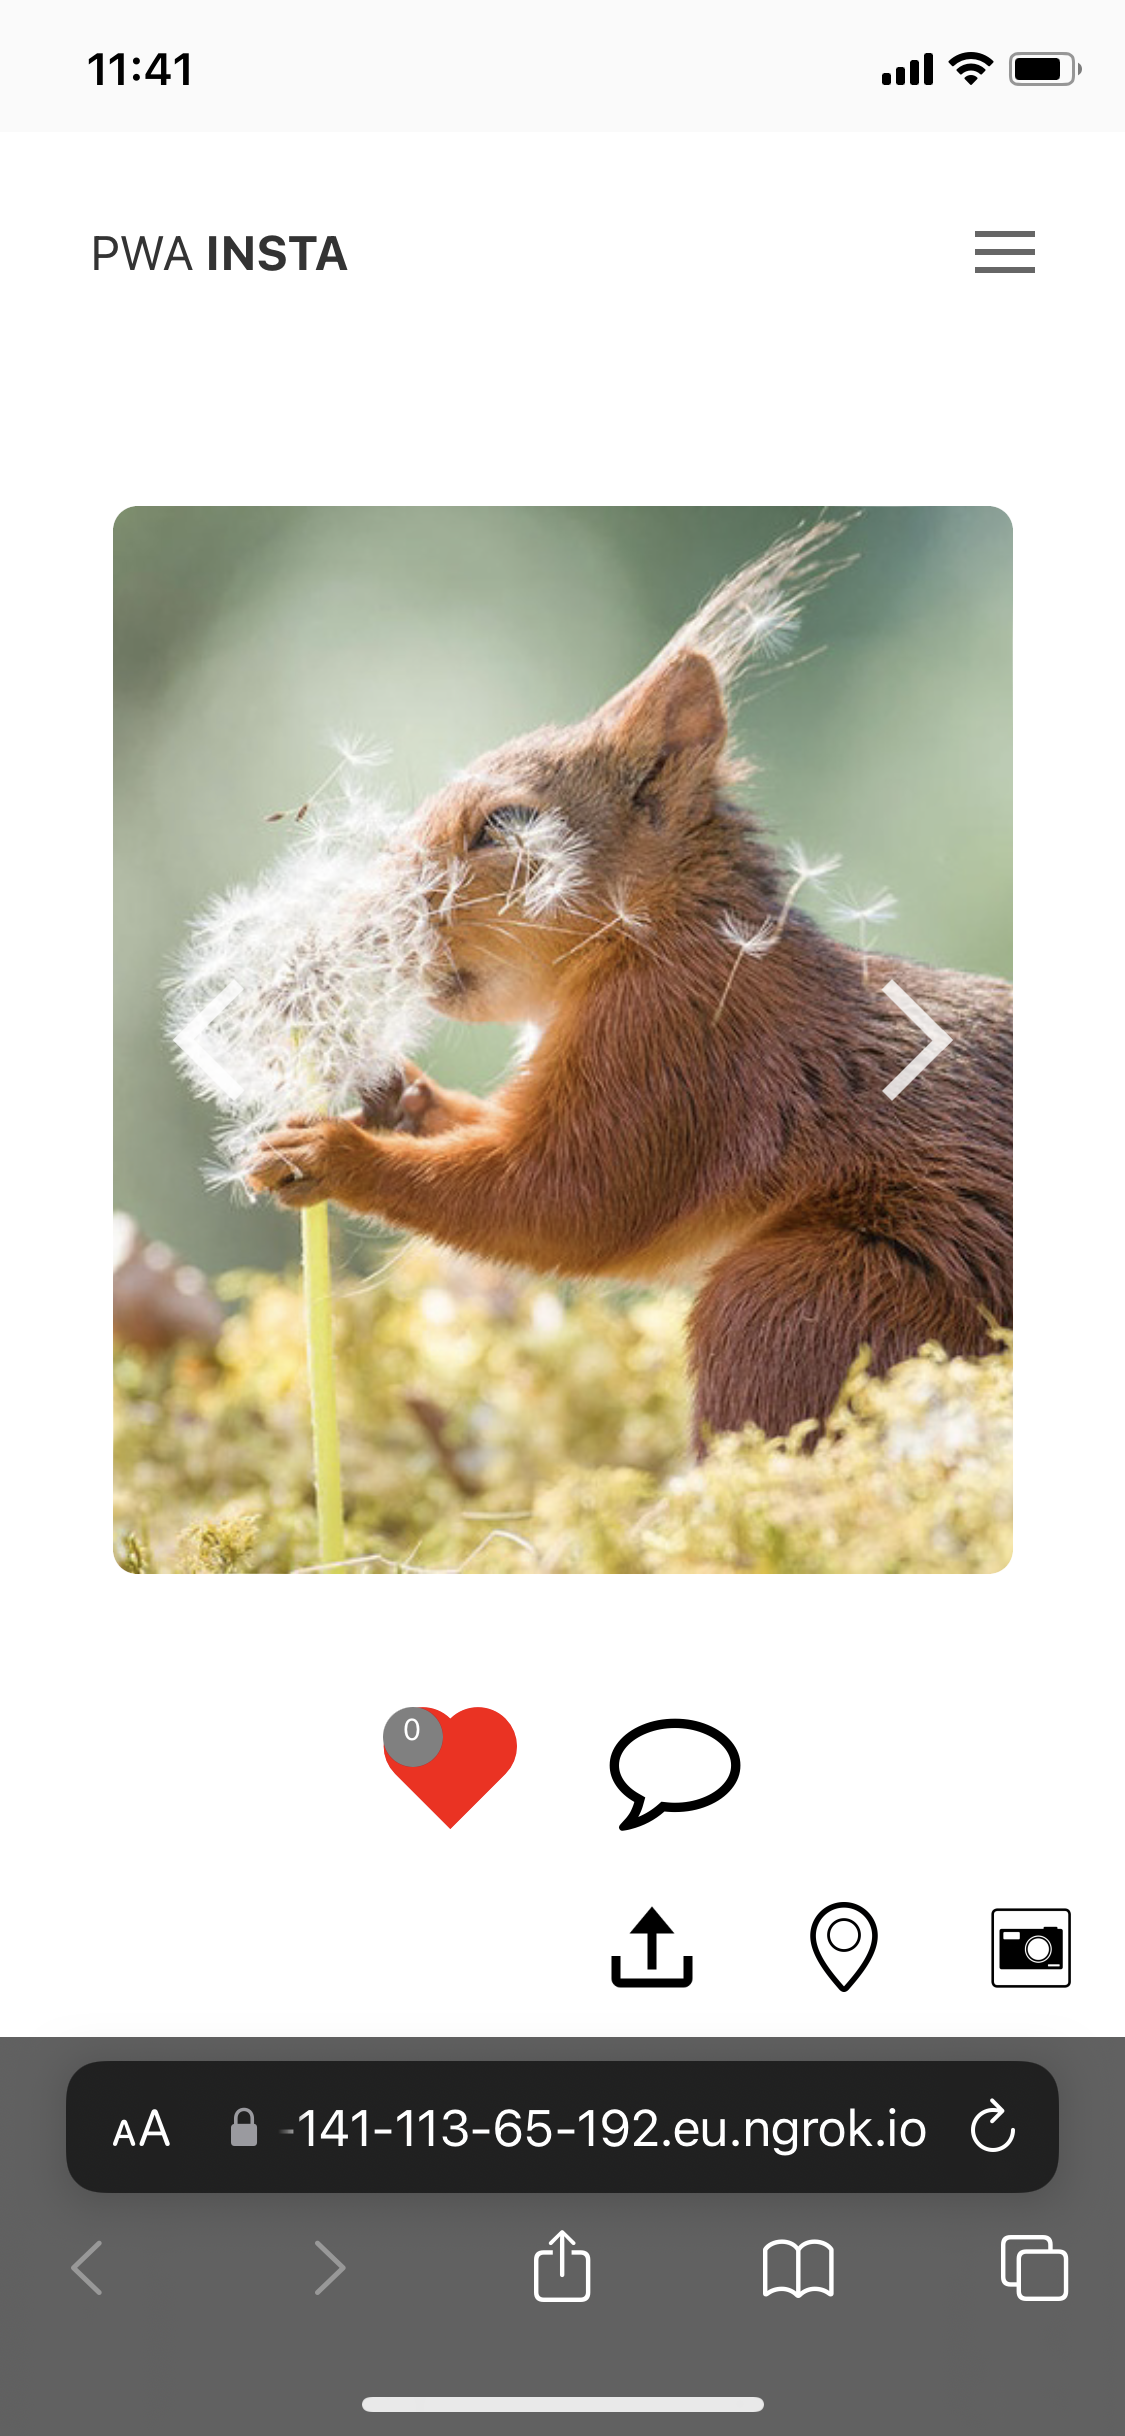
\includegraphics[width=\linewidth]{Iphone01.PNG}
       \caption{PWA im Apple Safari Browser in einem IOS System}
       \label{img:iphone01}
    \end{minipage}
    \hspace{.1\linewidth}% Abstand zwischen Bilder
    \begin{minipage}[b]{.4\linewidth} % [b] => Ausrichtung an \caption
       \includegraphics[width=\linewidth]{iphone02.PNG}
       \caption{Installation der PWA über die Auswahl \textit{Zum Home-Bildschirm}}
    \end{minipage}
 \end{figure}

 \begin{figure}[!htb]
    \begin{minipage}[b]{.4\linewidth} % [b] => Ausrichtung an \caption
       \includegraphics[width=\linewidth]{iphone03.PNG}
       \caption{Eingabe einer Bezeichnung für die PWA-App}
    \end{minipage}
    \hspace{.1\linewidth}% Abstand zwischen Bilder
    \begin{minipage}[b]{.4\linewidth} % [b] => Ausrichtung an \caption
       \includegraphics[width=\linewidth]{iphone09.jpg}
       \caption{Die installierte PWA-App auf dem Home-Bildschirm eines IOS-Systems }
       \label{img:iphone0n}
    \end{minipage}
 \end{figure}



	%!TEX root = ../../main.tex
\chapter{Verwendung von Geräteschnittstellen}

Eine weitere Eigenschaft von PWAs ist der Zugriff auf Geräteschnittstellen. Um dies zu zeigen, wird die Geolocation- und Kameraschnittstelle implementiert.
Wird in der unteren Navigationsleiste das mittlere Symbol ausgewählt, nutzt die Webanwendung die Geolocation-Schnittstelle, um dem Anwender seinen Breiten- und Längengrad mitzuteilen. Da es sich hierbei um eine datenschutzkritische Funktion handelt, muss der Anwender der PWA die Erlaubnis erteilen, auf dem Standort zuzugreifen. 

Die Geolocation wird auf allen Plattformen korrekt angezeigt und exemplarisch im IOS-System in den folgenden Abbildungen \ref{img:geo1} und \ref{img:geo2} gezeigt. 

\begin{figure}[!htb]
    \begin{minipage}[b]{.4\linewidth} % [b] => Ausrichtung an \caption
       \includegraphics[width=\linewidth]{Iphone05.PNG}
       \caption{Einholen der Nutzererlaubnis für den Zugriff auf den aktuellen Standort}
       \label{img:geo1}
    \end{minipage}
    \hspace{.1\linewidth}% Abstand zwischen Bilder
    \begin{minipage}[b]{.4\linewidth} % [b] => Ausrichtung an \caption
       \includegraphics[width=\linewidth]{iphone06.PNG}
       \caption{Darstellung des aktuellen Standorts in einer IOS-Anwendung}
       \label{img:geo2}
    \end{minipage}
 \end{figure}

 Die Anwendung implementiert auch die Kameraschnittstelle, welche ebenfalls auf allen Plattformen, die auf eine Kamera zugreifen können, funktioniert. Der Anwender muss auch für diese Funktion sein Einverständnis geben. Die Kamera-Funktion ist über das Kamera-Icon in der unteren Navigationsleiste erreichbar und wird in den folgenden Abbildungen \ref{img:Kamera1} und \ref{img:Kamera2} unter IOS dargestellt.

 \begin{figure}[!htb]
    \begin{minipage}[b]{.4\linewidth} % [b] => Ausrichtung an \caption
       \includegraphics[width=\linewidth]{Iphone07.PNG}
       \caption{Einholen der Nutzererlaubnis für den Zugriff auf die Kamera}
       \label{img:Kamera1}
    \end{minipage}
    \hspace{.1\linewidth}% Abstand zwischen Bilder
    \begin{minipage}[b]{.4\linewidth} % [b] => Ausrichtung an \caption
       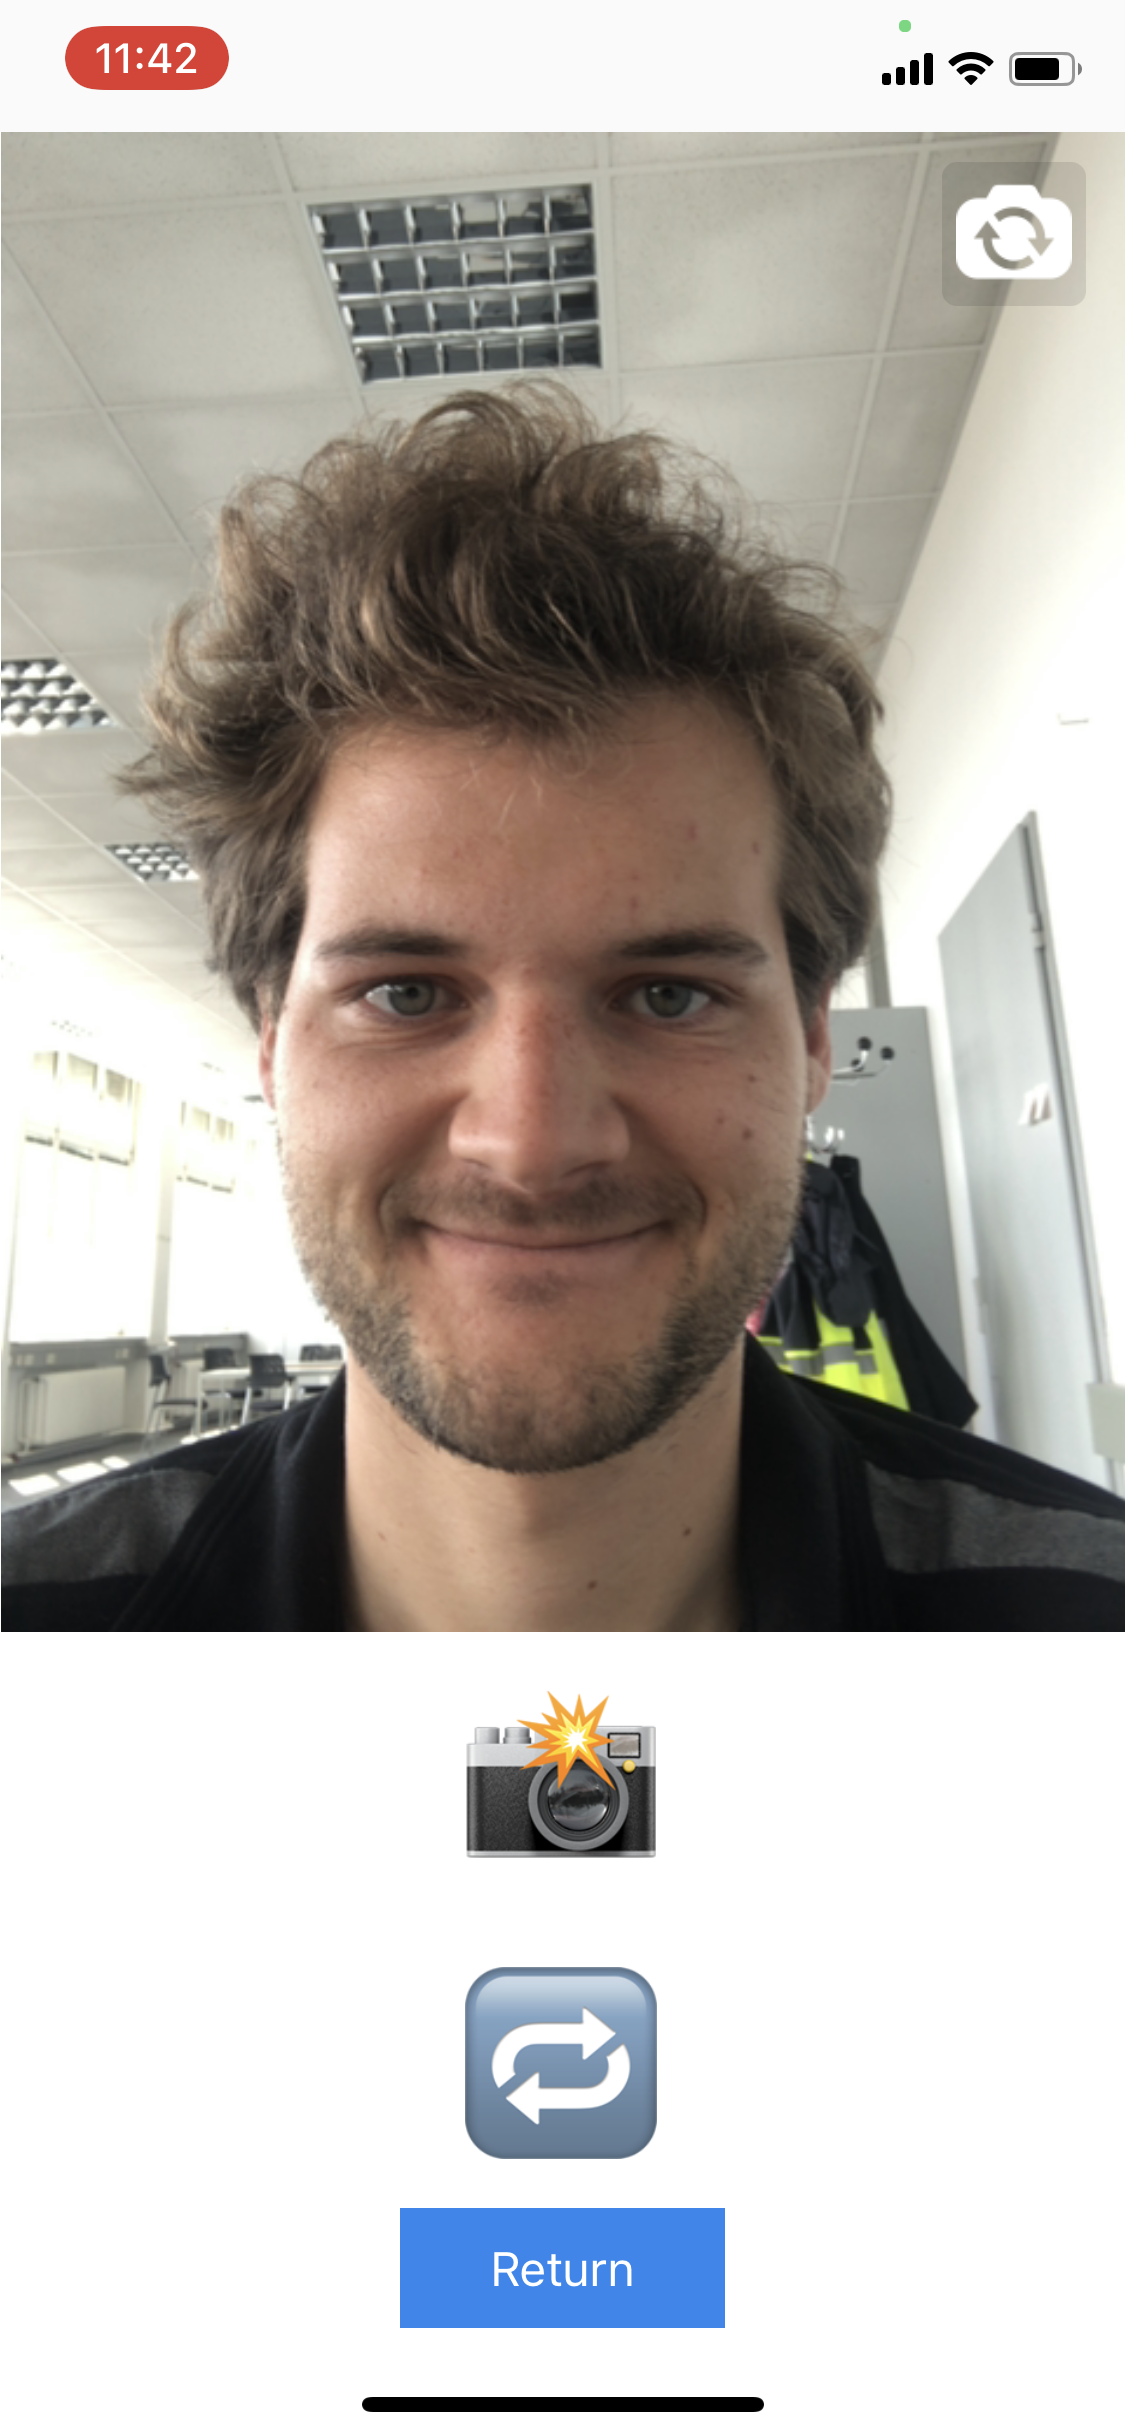
\includegraphics[width=\linewidth]{iphone08.PNG}
       \caption{Darstellung der Kamera-Funktion unter IOS}
       \label{img:Kamera2}
    \end{minipage}
 \end{figure}



	%!TEX root = ../../main.tex
\chapter{Push-Notifikation}\label{ch:PushNotifikation}

\section{Registrierung}

Damit die Webanwendung Push-Nachrichten empfangen kann, muss sie sich vorab beim Push-Dienst registrieren. Die Registrierung erfordert das Einverständnis des Anwenders. 
Um das Anwendererlebnis zu verbessern, wird dieser nicht direkt danach gefragt sondern kann über den Button \texttt{SUBSCRIBE TO PUSH} die Registrierung anstoßen, siehe Abbildung~\ref{img:permissionPush}. Um das Konzepte von Progressive Enhancement einzuhalten, wird der Button nur den Nutzern angezeigt, dessen Browser über die nötigen Funktionalitäten verfügt um Push-Nachrichten empfangen zu können. Hierfür wird der Button über eine \texttt{*ngIf}-Strukturdirektive ein- bzw ausgeblendet (Abschitt \ref{sec:Strukturdirektive}), je nach dem, ob der Browser über ein \texttt{PushManager} verfügt oder nicht. 

\begin{figure}[!htb]
    \centering
    \includegraphics[scale=0.4]{permissionPush.png}
    \caption{Nutzerabfrage um Push-Nachrichten versenden zu können. Abfrage erfolgt erst nachdem der Button \texttt{SUBSCRIBE TO PUSH} in der oberen Navigationsleiste ausgewählt wurde.}
    \label{img:permissionPush}
\end{figure}

Der Button ist mithilfe eines Event Bindings (Abschitt \ref{subsec:eventBinding}) an die Funktion \linebreak\texttt{subscribeToNotifications()} verknüpft. Da es sich bei der Anwendung um ein Angluar Projekt handelt, 
wird die Registrierung über die \texttt{SwPush}-Klasse durchgeführt (Listing \ref{lst:subscribeFkt} Zeile 2) die mithilfe von dependency injection über den Konstruktor geladen wurde. Wie in Abschnitt \ref{sec:pushRegistrirung} beschrieben wird die Push-Kommunikation durch das VAPID-Protokoll verschlüsselt. Hierfür muss bei der Registrierung der öffentliche Schlüssel übergeben werden (Listing \ref{lst:subscribeFkt} Zeile 3). Anders als in Abschnitt \ref{sec:pushRegistrirung} beschrieben, ist der Standartwert der Eigenschaft \texttt{userVisibleOnly}, aus dem Konfigurationsobjekt, \texttt{true}. Diese Einstellung wird von der Klasse \texttt{SwPush} vorgenommen. 

Ist die Registrierung erfolgreich wird ein Objekt von typ \texttt{PushSubscription} zurückgegeben. 
Das Objekt verfügt über folgende Eigenschaften: 
\begin{itemize}
    \item \textbf{endpoint}: Hinter dieser Eigenschaft befindet sich eine einzigartige URL, die für die Kommunikation mit dem Push-Dienst verwendet wird. 
    \item \textbf{expirationTime}: Durch diese Eigenschaft können Nachrichten versendet werden, die nur für einen bestimmten Zeitraum gelten. 
    \item \textbf{keys}: Enthält Informationen, um die Nachrichten zu entschlüsseln. 
\end{itemize}
Dieses Objekt muss im Anschluss über ein HTTP-Request an das Backend gesendet werden (Listing \ref{lst:subscribeFkt} Zeile 7-8). Hierbei wird die Kommunikation mit dem Backend in einem \texttt{Service} Ausgelagert. 

Falls die Registrierung erfolglos war, wird in der \texttt{catch}-Methode des Promises der Fehler auf der Konsole ausgegeben (siehe Listing \ref{lst:subscribeFkt} Zeile 11). 

Nach der Registrierung und dem Versenden des \texttt{PushSubscription} Objektes an das Backend müssen keine weiteren Vorkehrungen im Frontend vorgenommen werden. 

\begin{lstlisting}[caption={Funktion zur Registrierung beim Push-Dienst},label = lst:subscribeFkt,  float=!htb]
subscribeToNotifications(){
    this.swPush.requestSubscription({
      serverPublicKey: this.VAPID_PUBLIC_KEY
    })
      .then(subscribeObj => {
        console.log(subscribeObj);
        this.pushService.addPushSubscriber(subscribeObj).subscribe(res => {
          console.log('Backend Response Push Subscription' + res);
        });
      })
      .catch(err => console.error("Could not subscribe to notifications", err));
  }
\end{lstlisting}

\newpage
\section{Push-Nachrichten im Backend}

Im Backend werden zwei \texttt{post}-Endpunkte implementiert. Der Subscription Endpunkt wird verwendet, um das \texttt{PushSubScription} Objekt entgegenzunehmen. Das Objekt wird in einer Datenbank gespeichert. 

Der zweite Endpunkt wird verwendet um Push-Notifikations anzustoßen. Das Backend benutzt die Web-Push Bibliothek um allen Registrierten Klienten eine Push-Nachricht zu senden.  Die \texttt{sendNotifikation}-Methode der Web-Push Bibliothek benötigt ein Payload und ein \texttt{PushSubScription}-Objekt. Im Payload werden die Informationen angegeben, die in der Push-Nachricht angezeigt werden, hierbei muss mindestens ein Title und eine Nachricht vorhanden sein, siehe Listing \ref{lst:payload}. 

\begin{lstlisting}[caption={Mindestanforderung an ein Payload, für eine Push-Nachricht}, label=lst:payload, float=!htb]
    const notificationPayload = {
        notification: {
            title: 'Neue Notification',
            body: 'Das ist der Inhalt der Notification'
        },
    }
\end{lstlisting}

Die Web-Push Methode, verschlüsselt die Nachricht vor dem Versenden, hierfür müssen die VAPID-Schlüsselpaare der Methode \texttt{webpush.setVapidDetails()} übergeben werden. 
Wird nun eine HTTP-Post Anfrage an diesen Endpunkt gesendet, iteriert die Funktion über alle in der Datenbank gespeicherten \texttt{PushSubscription}-Objekte und sendet über die \texttt{sendNotifikation}-Methode den verschlüsselten Payload. Alle registrierten Klienten erhalten folgende Mitteilung, siehe Abbildung \ref{img:notificationBanner}.

\begin{figure}[!htb]
    \centering
    \includegraphics[scale=0.7]{notificationBanner.png}
    \caption{Push-Nachricht, mit dem Payload aus Listing \ref{lst:payload}}
    \label{img:notificationBanner}
\end{figure}
	%!TEX root = ../../main.tex
\chapter{Bewertung der Plattformunabhängigkeit}

Apple unterstützt die Entwicklung von PWAs nicht. PWAs stellen  eine Möglichkeit dar, um Apps für das iPhone zu installieren, die sich nicht in dem App Store befinden. Im Jahr 2020 hat Apple mit dem App Store einen Umsatz von 643 Milliarden US-Dollar erwirtschaftet \cite{Kirchenbauer2021}. Apple erhält 30\% Provision, wenn Apps gekauft oder In-App-Käufe abgeschlossen werden. Durch den Einsatz von PWAs könnte diese Einnahmen reduziert werden.

Google ist maßgeblich an der Entwicklung von PWAs beteiligt. Dementsprechend Funktionieren PWAs im Google-Ökosystem am besten. Besonders gut ist die Unterstützung von PWAs bei der Installation zu beobachten. In Google Chrome wird nur ein Klick auf den sehr präsenten Button in der Suchleiste benötigt und unter Android wird den Anwender aktiv gefragt ob er die PWA installieren möchte. Auch sämtliche Funktionen wie Push-Notifications, Caching und Geräteschnittstellen werden vollumfänglich unterstützt. 
Google unterstützt nicht nur die Anwender von PWAs sondern auch die Entwickler. In dem von Google entwickelten Webframework Angular benötigt es nur wenige befehle um eine bereits existierende Angular-Webanwendung in eine PWA zu erweitern. 

Obwohl PWAs nicht vollumfänglich im Apple-Ökosystem verwendet werden können sind wir dennoch davon überzeugt, das sie in Zukunft immer mehr an Bedeutung gewinnen werden. Durch die Entwicklung einer PWA waren wir in der Lage eine Anwendung für den Rechner, Web und das Smartphone zu entwickeln und zu installieren. Als Programmiersprache wurde JavaScript verwendet. JavaScript ist laut der Umfrage von Stack Overflow bereits seit neun Jahren im Folge die beliebteste Programmiersprache. Im Jahr 2021 haben 64\% der befragten Entwickler angegeben JavaScript zu verwenden.
Im Gegensatz verwendeten nur 35\% Java, 27\% C\# und 5\% Swift \cite{stackoverflow2021}. 




	
	\clearpage

	% Bibilography
	\cleardoublepage
	\printbibliography

	% Glossar
	\cleardoublepage
	\printglossary[style=altlist,title=\glossaryPhrase]
	\input{content/glossary}
	
	% Appendix
	\clearpage
	\appendix
	% !TeX root = ../main.tex

\addchap{\appendixPhrase}

\section{HTML} \label{sec:html}
Mit der \ac{HTML} wird das Grundgerüst einer Internetseite aufgebaut. Dafür werden Textelemente von einem HTML-Tag jeweils geöffnet (<html>) und geschlossen (</html>).  Auch HTML-Tags können Einfluss auf die Position und die Darstellung der Textelemente im Browser ausüben. Zum Beispiel verursacht der HTML-Tag \texttt{<h1>Text</h1>}, dass das Textelement als Überschrift angezeigt wird \cite{W3HTML2021}. 

Eine HTML-Datei verfügt im Allgemeinen über folgendes Grundgerüst.

\begin{lstlisting}[caption=Grundgerüst einer HTML-Seite, label=htmlGrundgerüst]
<!DOCTYPE html>
<html>
    <head>
        <title>Seitentitel</title>
    </head>
    <body>
        <h1> Das ist eine Grosse Ueberschrift </h1>
        <p> Das ist ein Absatz </p>
    </body>
</html>
\end{lstlisting}

Der Tag \texttt{<!DOCTYPE html>} gibt dem Browser an, dass es sich um eine HTML-Datei handelt. Der \texttt{<head>}-Bereich beinhaltet Metadaten über das Webdokument, wie zum Beispiel den Titel, der im Browser-Reiter angezeigt wird. Neben dem Titel können im Head noch weitere Metadaten wie Schlüsselwörter, Autor und Zeichenkodierung angegeben werden. Wird das Aussehen einer Webseite in einer separaten Datei festgelegt, muss diese Datei auch im Head der HTML-Datei verlinkt werden. Die Inhalte, die vom Browser dargestellt werden, sind im \texttt{<body>}-Bereich angegeben. Im Code-Beispiel \ref{htmlGrundgerüst} ist das eine Überschrift und ein Absatz und wird, wie in Abbildung \ref{img:htmlGrund} dargestellt, im Browser angezeigt.

\begin{figure}[!htb]
    \centering
    \includegraphics[scale=0.5]{htmlGrund.png}  
    \caption{HTML Grundgerüst}
    \label{img:htmlGrund}
\end{figure}

\subsection{Attribute} \label{sec:Attribute}

HTML-Tags können durch Attribute erweitert werden. Die Attribute werden innerhalb der spitzen Klammern angegeben, siehe Listing \ref{list:htmlAttribut}. Besonders wichtig sind globale Attribute, die für alle HTML-Elemente verwendet werden können. Mithilfe des globalen Attributs \texttt{class} können mehrere HTML-Tags in einer Kategorie beziehungsweise Klasse zusammengefasst werden. Die Eigenschaften dieser Klasse können im Anschluss in der CSS-Datei beeinflusst werden, siehe das folgende Kapitel.

\begin{lstlisting}[caption=HTML Attribute, label=list:htmlAttribut]   
<h1 class="Ueberschrift"> 
    Das ist eine Grosse Ueberschrift 
</h1>
\end{lstlisting}


%--------------------------------------
\section{CSS} \label{sec:css}

\ac{CSS} werden verwendet, um 
\begin{itemize}
    \item dem HTML-Dokument einen ansprechenden Stil zuzuweisen,
    \item das Layout des HTML-Dokumentes zu definieren und
    \item das Layout so zu gestalten, dass sich der Inhalt automatisch an die Bildschirmgröße anpasst. 
\end{itemize}

Generell gilt, dass mit HTML die Inhalte definiert werden und mit CSS das Aussehen. 
Die Syntax, um CSS-Eigenschaften für HTML-Elemente zu definieren, ist wie folgt aufgebaut. 

\begin{lstlisting}[caption= Die generelle Syntax für CSS-Eigenschaften, label=syntaxCSS]
selektor {
    Eigenschaften : Wert;
}
\end{lstlisting}

Selektoren können HTML-Elemente wie \texttt{<h1>} und \texttt{<p>}, oder Klassen und IDs, wie bereits im Kapitel \ref{sec:html} angesprochen, sein. Wird eine Klasse als Selektor verwendet, muss ein Punkt vor den Namen geschrieben werden, bei einer ID eine Raute \cite{W3CSS2021}.

Um die Überschrift aus Listing \ref{list:htmlAttribut} grün zu färben, würde die CSS-Syntax wie in Listing \ref{UeberschriftGruen} dargestellt, aussehen. Das Ergebnis ist in Abbildung \ref{img:UeberschriftGruen} dargestellt.  

\begin{lstlisting}[caption= Grüne Überschrift CSS, label=UeberschriftGruen]

<!-- eine Klasse als Selektor -->
.Ueberschrift {
    color : green;
}

<!-- ein HTML-Element als Selektor--> 
h1 {
    color : green;
}
\end{lstlisting}

\begin{figure}[!htb]
    \centering
    \includegraphics[scale=0.5]{gruenerUeberschrift.png}
    \caption{Grüne Überschrift}
    \label{img:UeberschriftGruen}
\end{figure}

\subsection{CSS in die HTML-Datei einbinden}

Wie im Kapitel \ref{sec:html} bereits erwähnt, ist es  möglich, eine CSS-Datei im HTML-Head zu verlinken, siehe Listing \ref{CSSLink}. Darin wird die Datei \textbf{style.css} eingebunden. 

\begin{lstlisting}[caption= CSS-Datei in HTML verlinken, label=CSSLink, float=!htb]
<head>
    <link rel="stylesheet" href="style.css">
</head>
<body>
    <h1 class="Ueberschrift"> 
        Das ist eine Grosse Ueberschrift 
    </h1>
</body>
\end{lstlisting}

Das Attribut \texttt{href} gibt den Pfad der verlinkten Ressource an. Die Beziehung des verknüpften Dokuments zum aktuellen Dokument wird mit dem Attribut \texttt{rel} angegeben \cite{Mozilla2021}.
CSS Deklarationen können auch direkt in das HTML Dokument geschrieben werden, indem man den HTML-Tag \texttt{<style>} verwendet, Listing \ref{CSSdirekt}. 

\begin{lstlisting}[caption= CSS-Datei in HTML einbinden, label=CSSdirekt]
<head>
    <style>
        .Ueberschrift {
            color : green;
        }
    </style>
</head>
<body>
    <h1 class="Ueberschrift"> 
        Das ist eine Grosse Ueberschrift 
    </h1>
</body>
\end{lstlisting}

%----------------------------------
\section{JavaScript}\label{sec:JavaScript}

JavaScript ist eine Programmiersprache, mit der man komplexe Funktionen für Webseiten realisieren kann. JavaScript findet immer dann Anwendung, wenn eine Internetseite mehr als nur statische Informationen darstellt \cite{Mozilla2021}. 

Mithilfe von JavaScript können: 
\begin{itemize}
    \item Informationen in Variablen gespeichert,
    \item Operationen auf Webinhalte, wie zum Beispiel Texte ausgeführt und 
    \item auf Ereignisse reagiert werden, wie zum Beispiel auf einen Maus-Klick.  
\end{itemize}

\subsection{JavaScript in die HTML-Datei einbinden}
JavaScript kann, genauso wie CSS, entweder unter Verwendung des HTML-Tags \texttt{<script>} direkt in das HTML-Dokument geschrieben werden, oder der Code wird als externe Datei eingebunden. Dafür wird auch der HTML-Tag \texttt{script} verwendet, mit dem Attribut \texttt{src}\footnote{source (Quelle)}, und dem Pfad der JavaScript Datei \cite{W3JS2021}, siehe Listing \ref{jsHTML}. 

\begin{lstlisting}[caption= JavaScript in HTML einbinden, label=jsHTML, float=!htb]
    <head>
        <!--direkte Einbindung -->
        <script>
           //JavaScript Code 
        </script>

        <!-- als externe Datei Einbinden -->
        <script src="dateiname.js"></script>
    </head>
\end{lstlisting}

	

\end{document}
